%------------------------------------------------- 
\subsection{Discovery Strategy)}
\label{subsec:fit_bh}

Model-independent fits for the discovery region will be performed using \href{https://github.com/scikit-hep/pyBumpHunter}{pyBumpHunter}.
The strategy will consist of comparing the data in a given \mt~spectrum of interest to a background estimation derived by performing the polynomial fit and sampling from the post-fit function into a histogram.
The polynomial fit is done to an \mt~distribution with 180 bins (25 GeV wide). %90 bins, as with the PFN \mt~spectrum.
To keep the trials factor moderate, a rebinning will be performed based on the signal mass resolution in \mt (Section~\ref{subsec:binning}) to best assess the significance of BumpHunter results.
This is under development with preliminary studies shown in Appendix~\ref{app:bumphunter}.

Figure~\ref{fig:postfit_param_antelope} shows the post-fit values of the fit parameters and their uncertainties for the discovery (ANTELOPE-based) CR and VR. 
Figure~\ref{fig:bkgfit_data_crvr_antelope} shows the resulting functions and residuals with respect to the CR and VR data.
These results indicate good ability of the 5-parameter polynomial to also model the ANTELOPE selected region.
\begin{figure}[!htbp]
\centering
   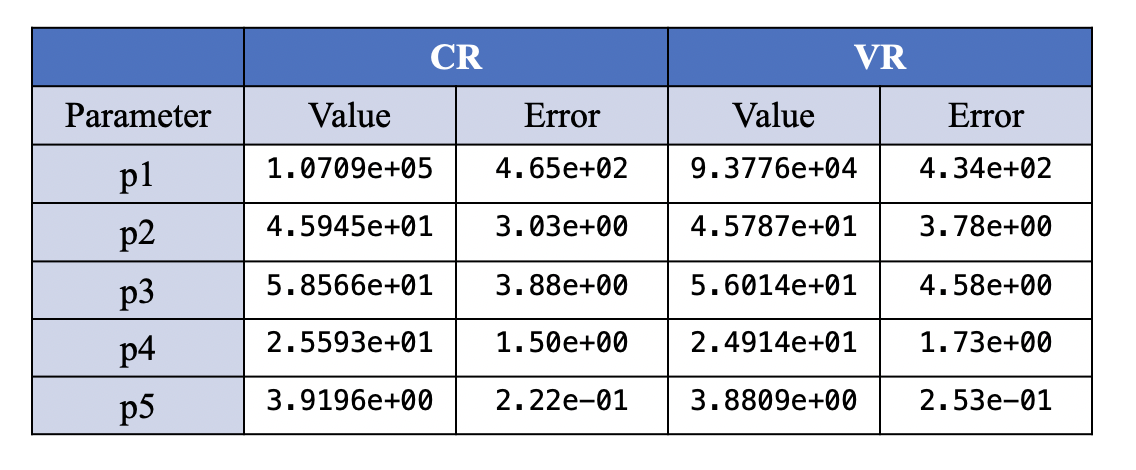
\includegraphics[width=0.65\textwidth]{figures/stats/postfit_param_antelope}
    \caption{Post-fit parameters for the ANTELOPE CR and VR.
    \label{fig:postfit_param_antelope}}
\end{figure}
\begin{figure}[!htbp]
\centering
   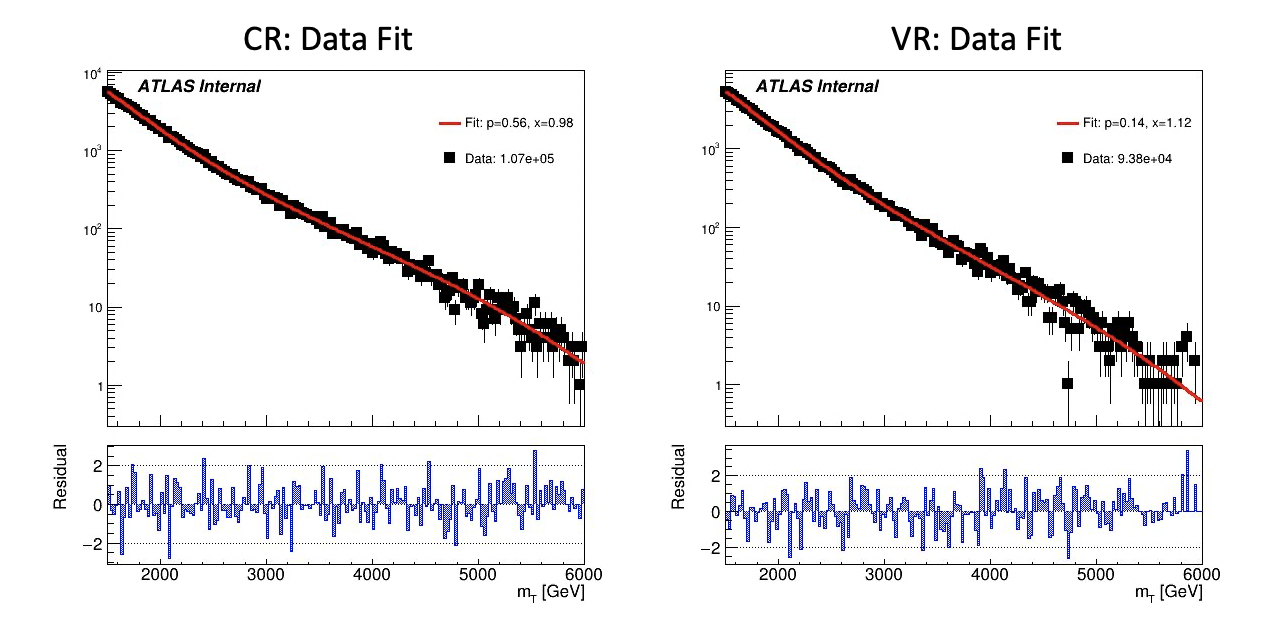
\includegraphics[width=0.95\textwidth]{figures/stats/bkgfit_data_crvr_antelope}
    \caption{Post-fit function and residuals for the ANTELOPE CR and VR.
    \label{fig:bkgfit_data_crvr_antelope}}
\end{figure}


%----------------------------------------------------------------------------------------
\subsubsection{Signal Mass Resolution \mt~Binning}
\label{subsec:binning}

In the discovery region, a binning for \mt~is determined that is based on the expected signal width. This is done to improved the BumpHunter performance.
The signal mass resolution for a given point is determined with a double-sided Crystal Ball fit to the mass. 
These fits are performed across Z' mass, and a linear fit to these values is performed to determine the optimal bin width across \mt.

The x-axis value used is a data-driven way to determine the appropriate value of \mt~for a given signal, given that the considerable \met~from the dark particles means that the truth Z' mass does not well approximate the peak \mt~value.
As the \met~in the final state means that the \mt~is always an underestimate of the Z' mass, the truth Z' mass can be used as an upper bound.
An integral is then performed backwards from that value until 60\% of the total signal yield is included. 
This window is referred to as the 60\% mass window; the mean of this window then provides an approximate localization of the signal mass peak in \mt.
Figure~\ref{fig:mass60percent_ex} shows some examples of this algorithm on several signal points of varying \rinv~and mass.
\begin{figure}[!htbp]
\centering
   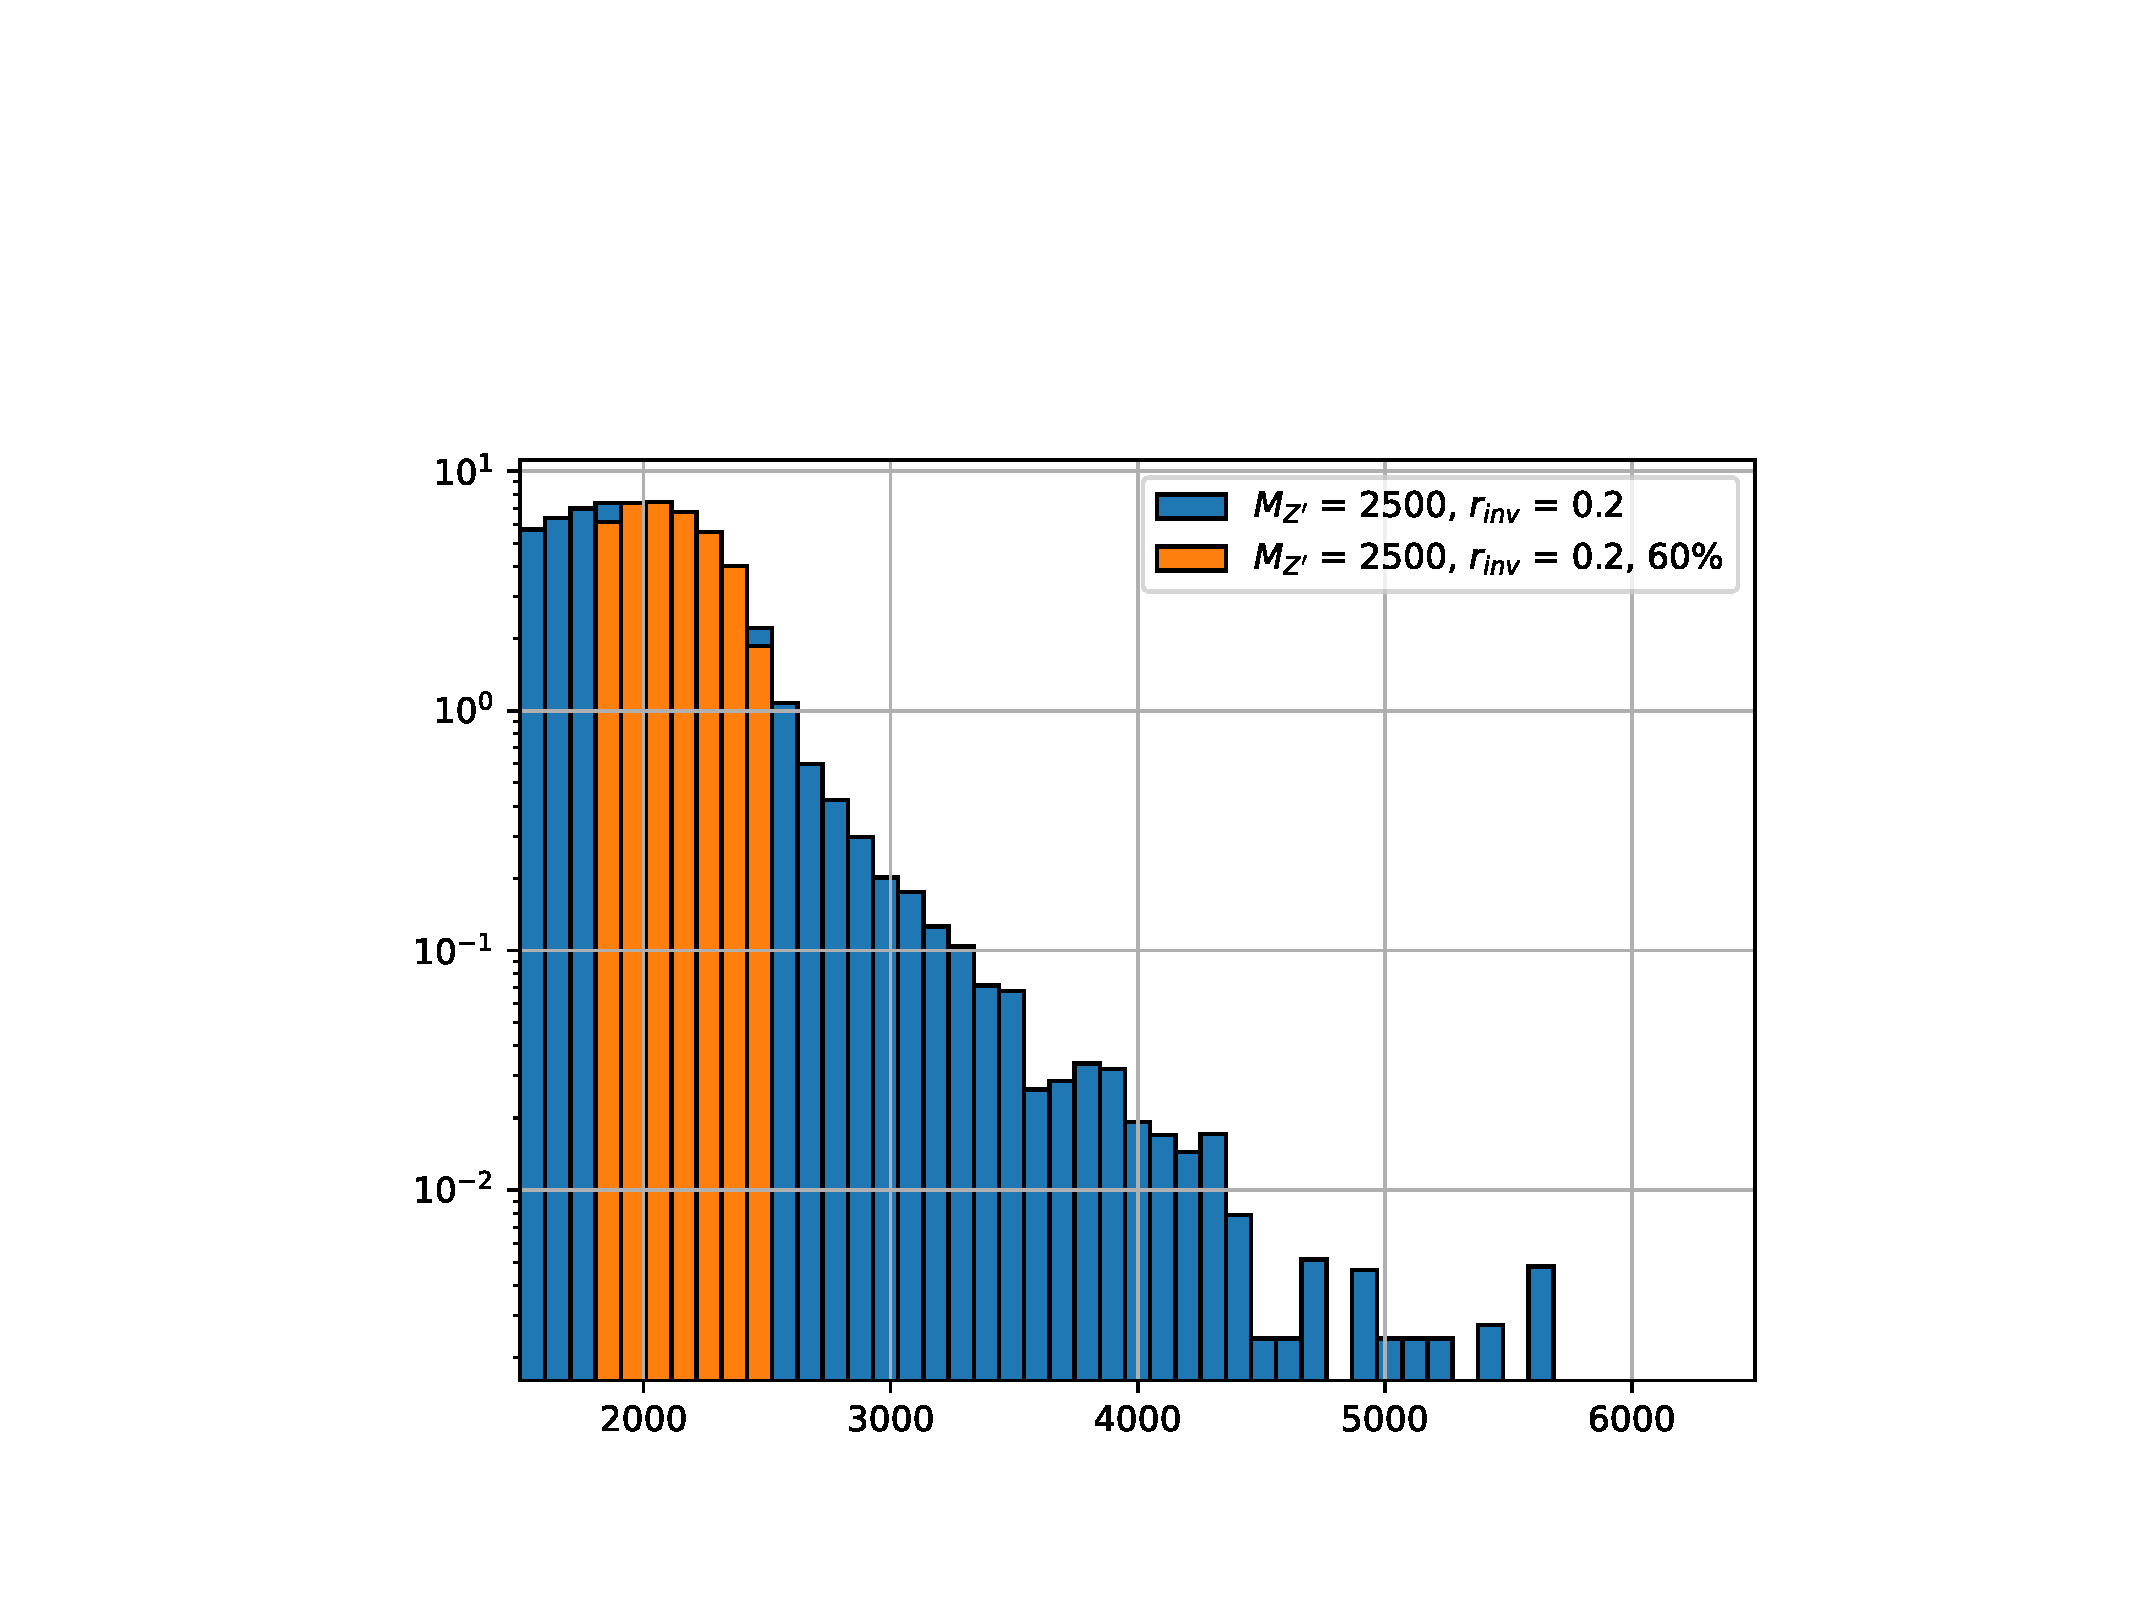
\includegraphics[width=0.45\textwidth]{figures/stats/mass60percent_ex1}
   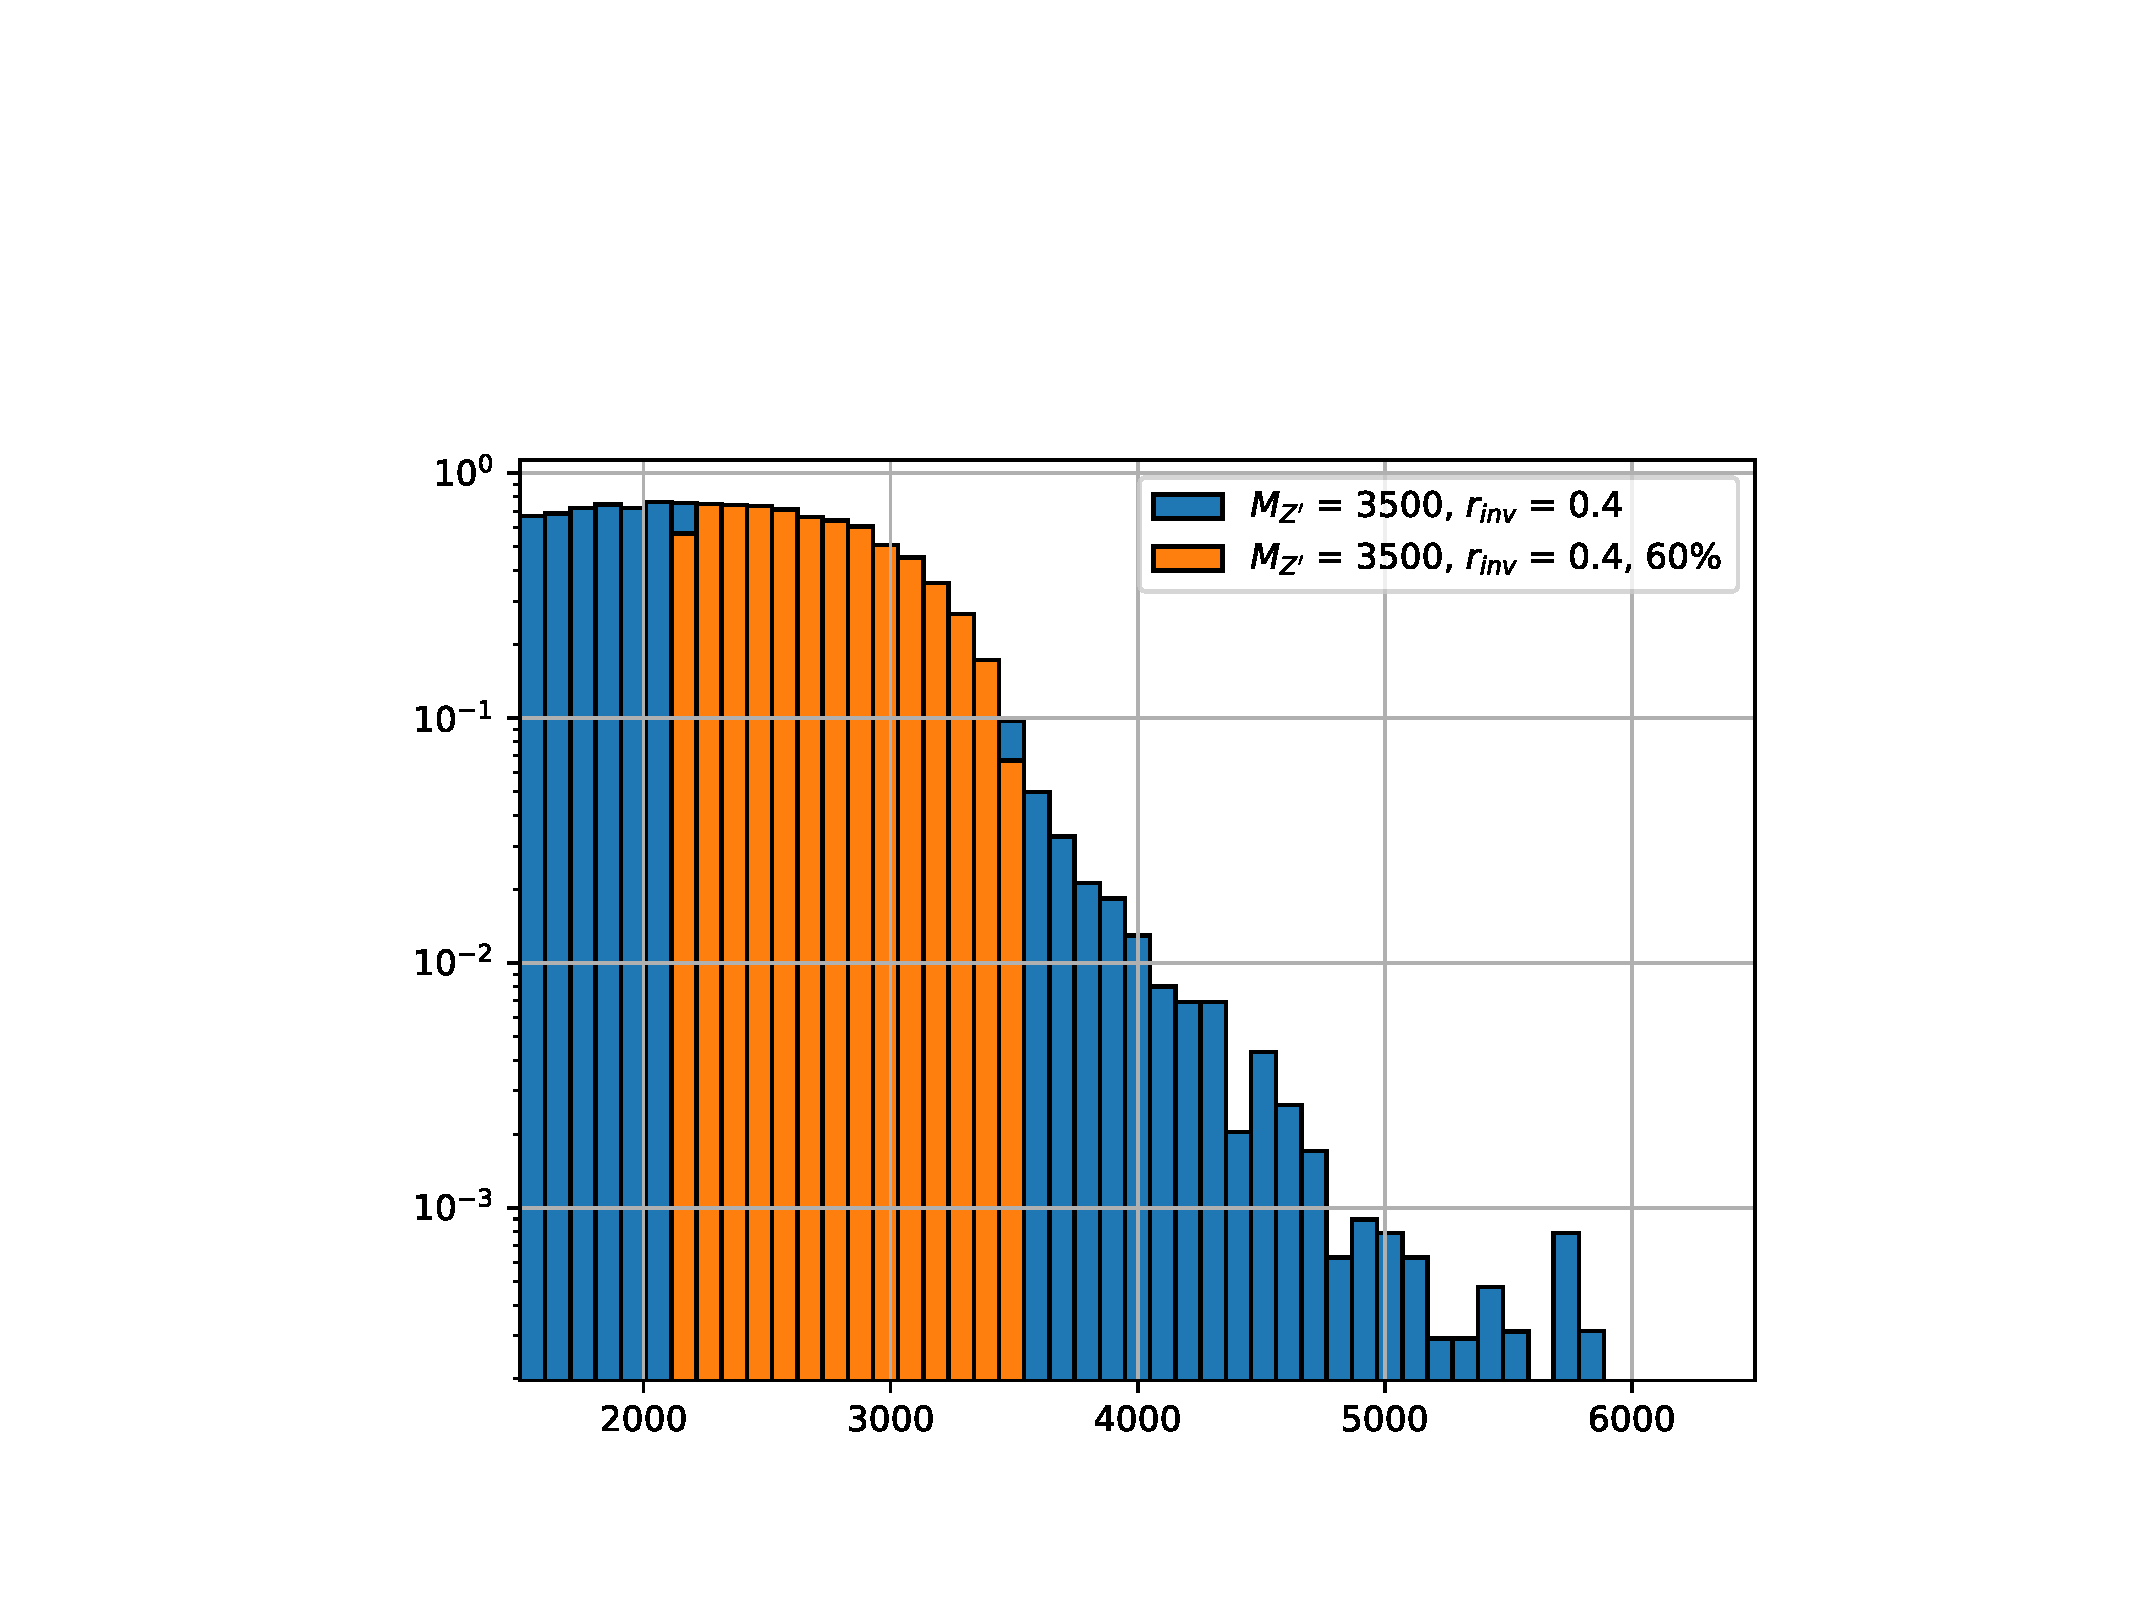
\includegraphics[width=0.45\textwidth]{figures/stats/mass60percent_ex2}
   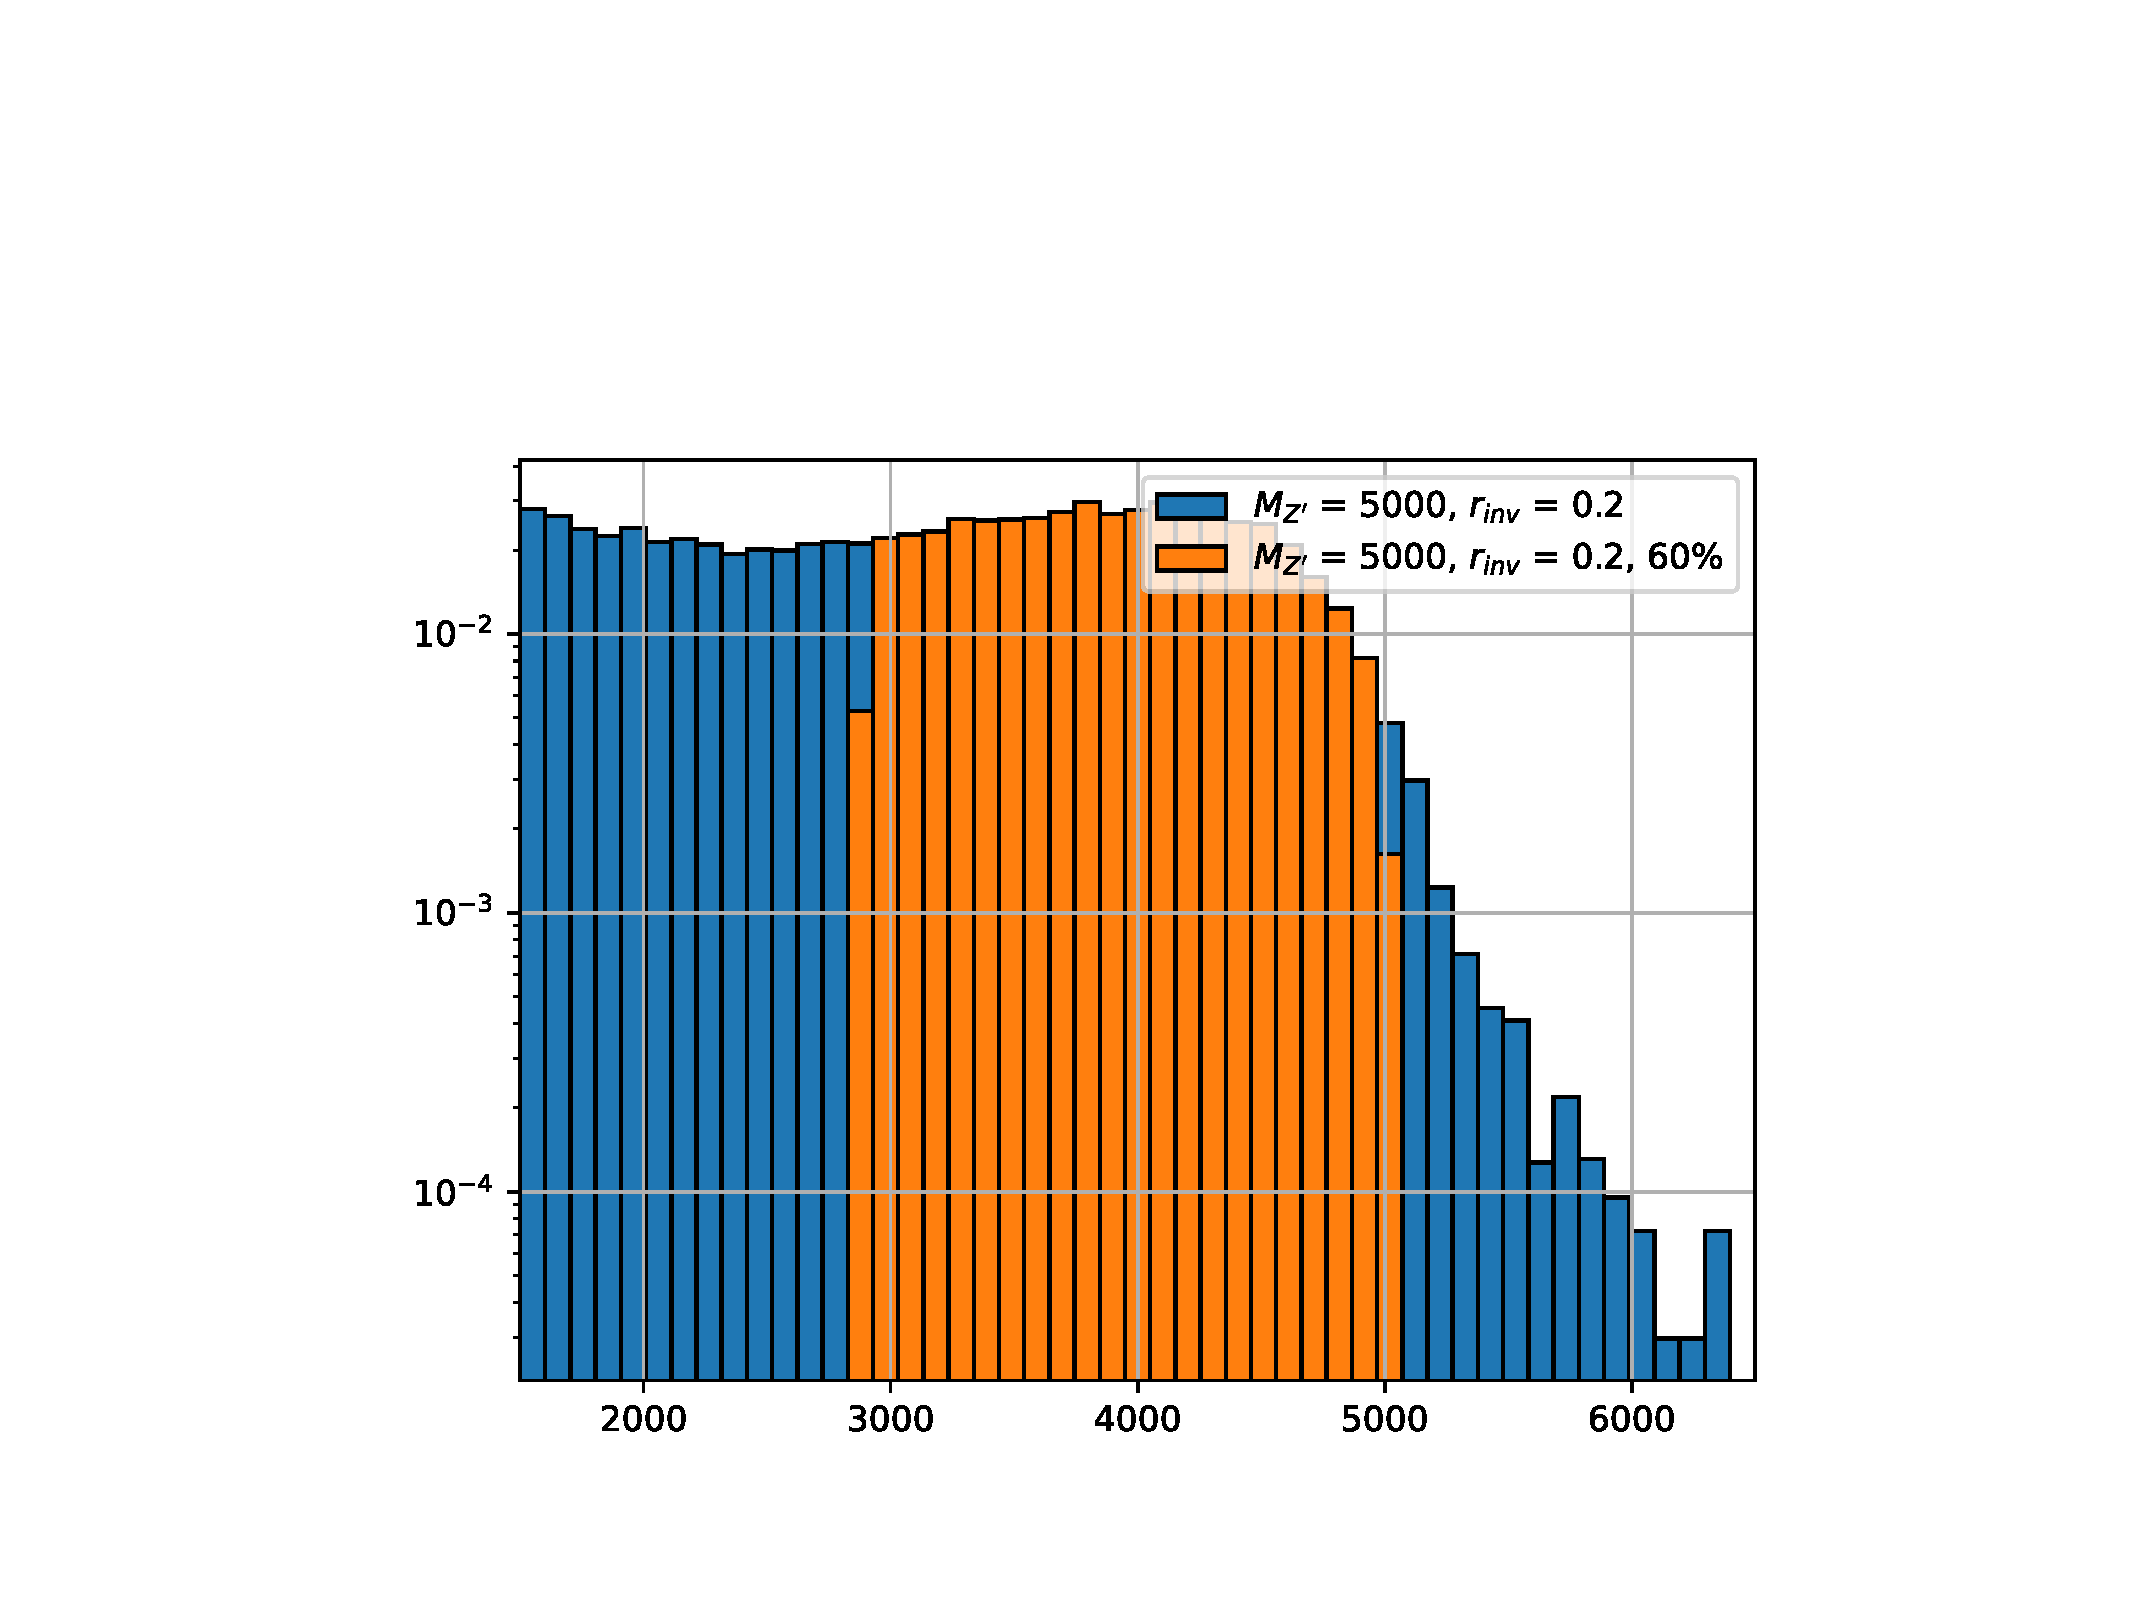
\includegraphics[width=0.45\textwidth]{figures/stats/mass60percent_ex4}
   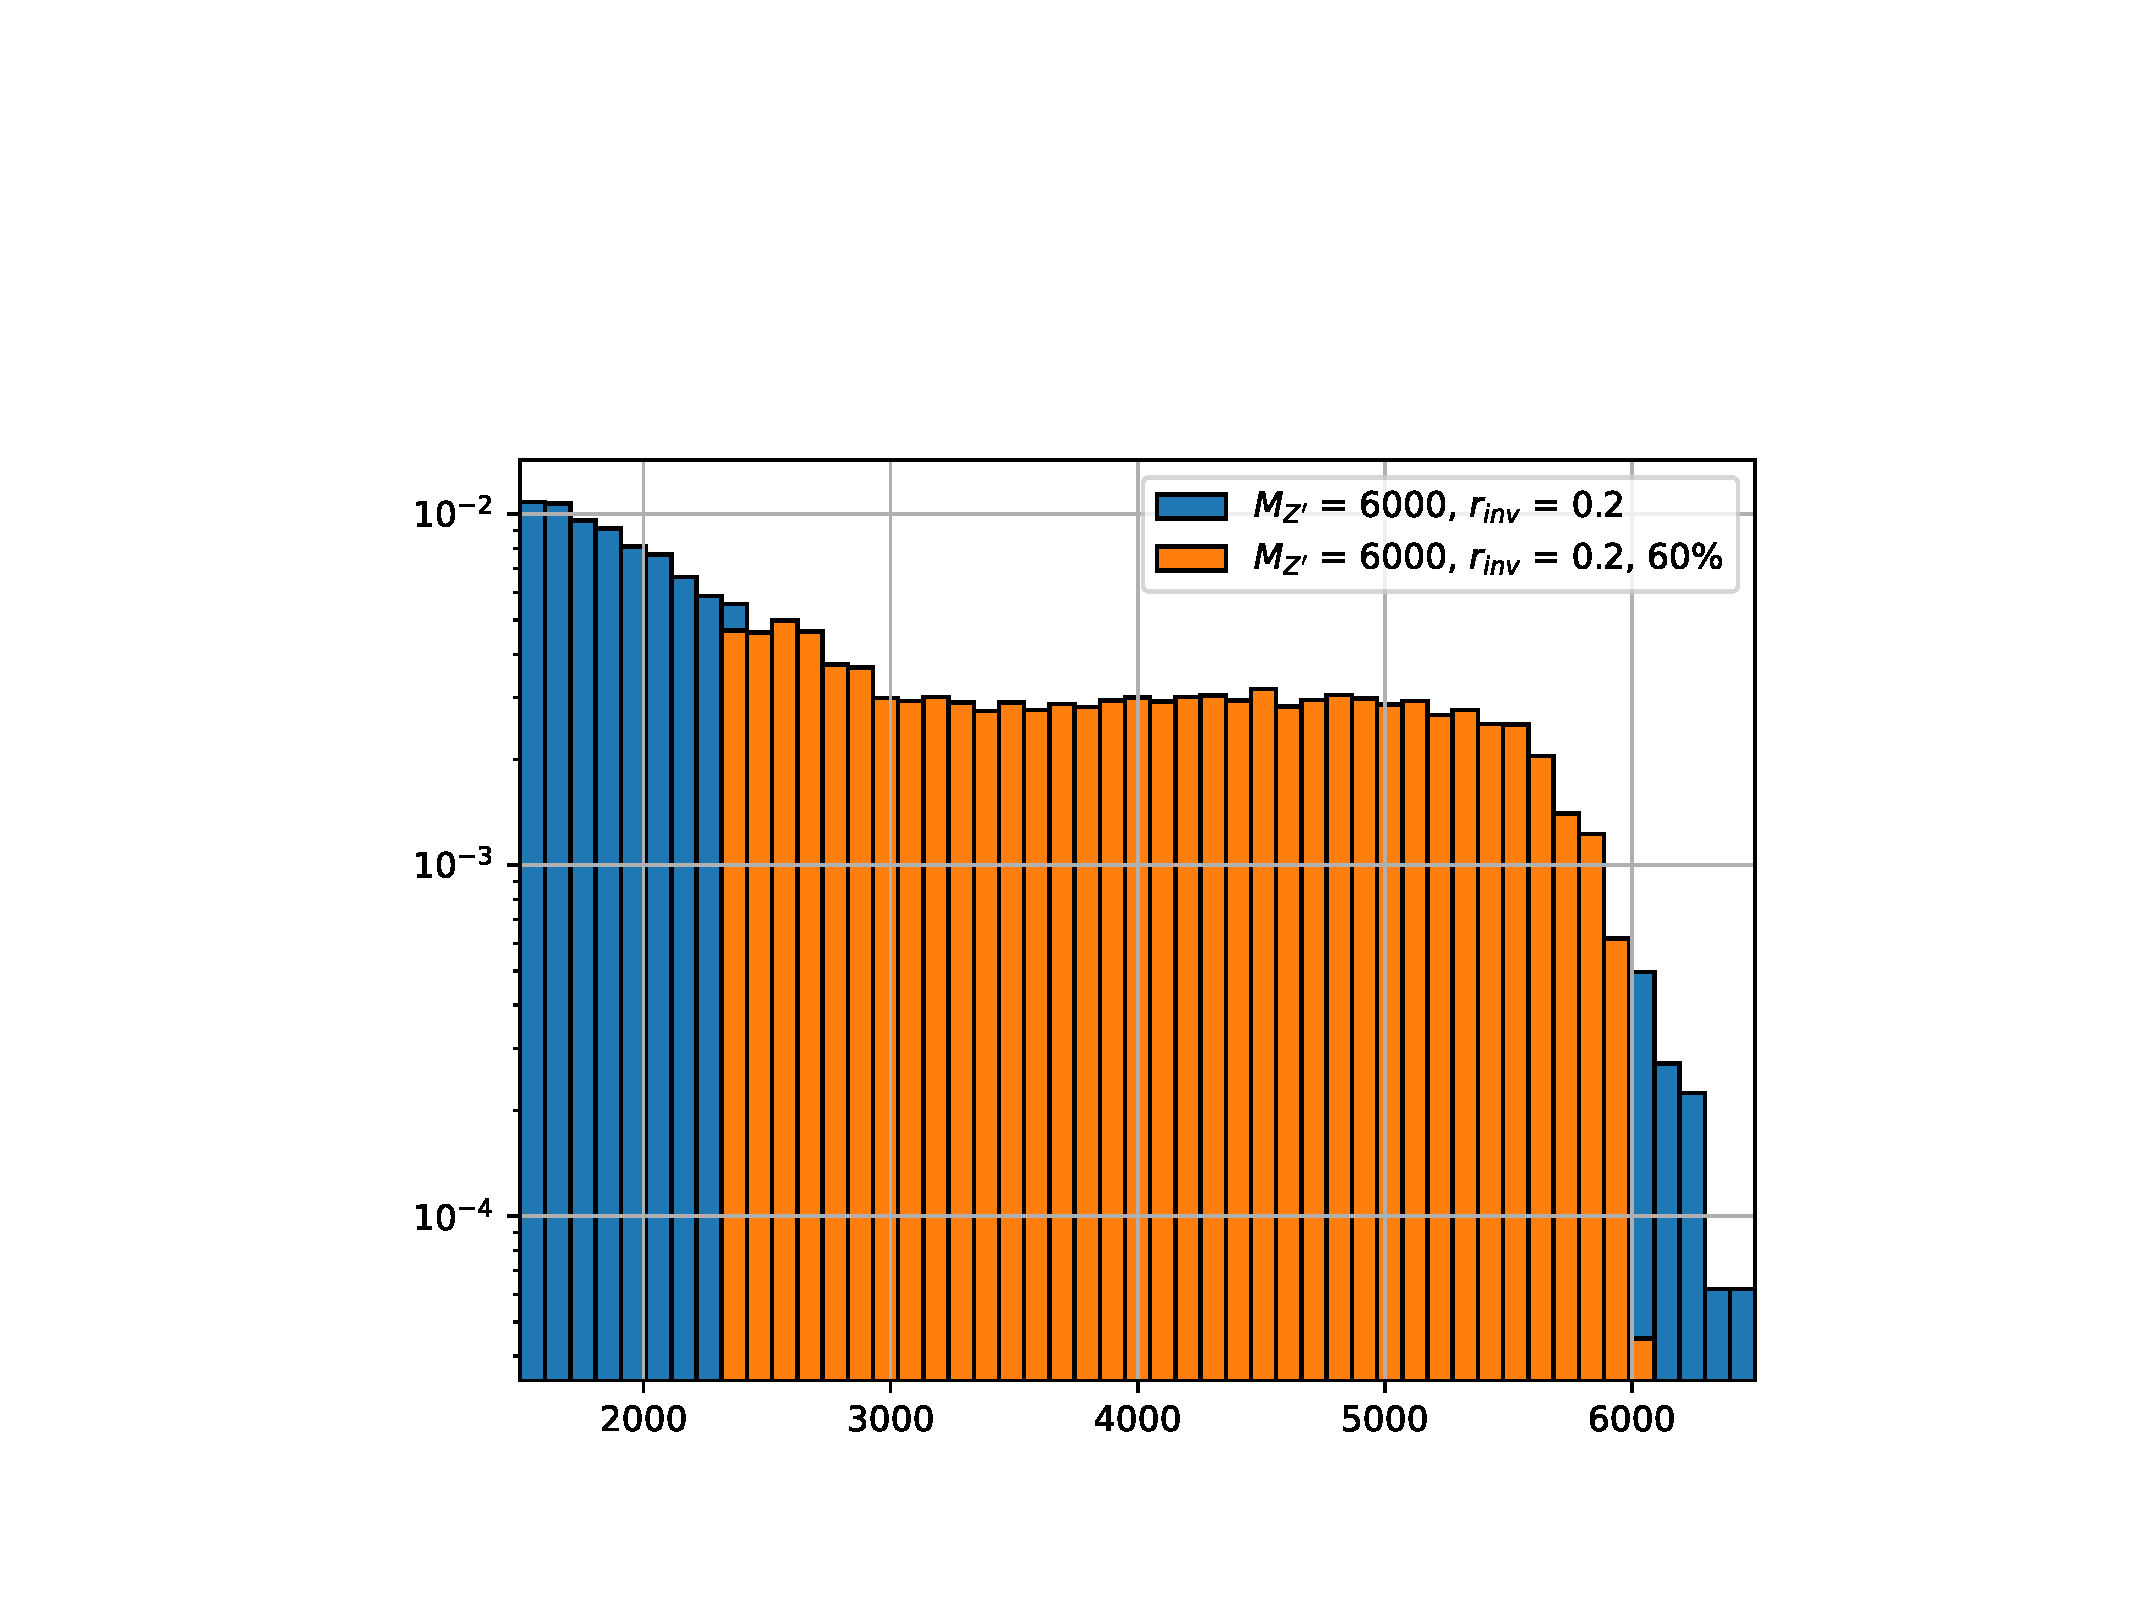
\includegraphics[width=0.45\textwidth]{figures/stats/mass60percent_ex3}
    \caption{Example determinations of the 60\% mass window means for several signal points.
    \label{fig:mass60percent_ex}}
\end{figure}

Figure~\ref{fig:linearfit_binning} shows the result of this linear fit for the four \rinv~values considered in the signal grid.
As expected, the resolution is considerably different for low and high \rinv~points.
\begin{figure}[!htbp]
\centering
   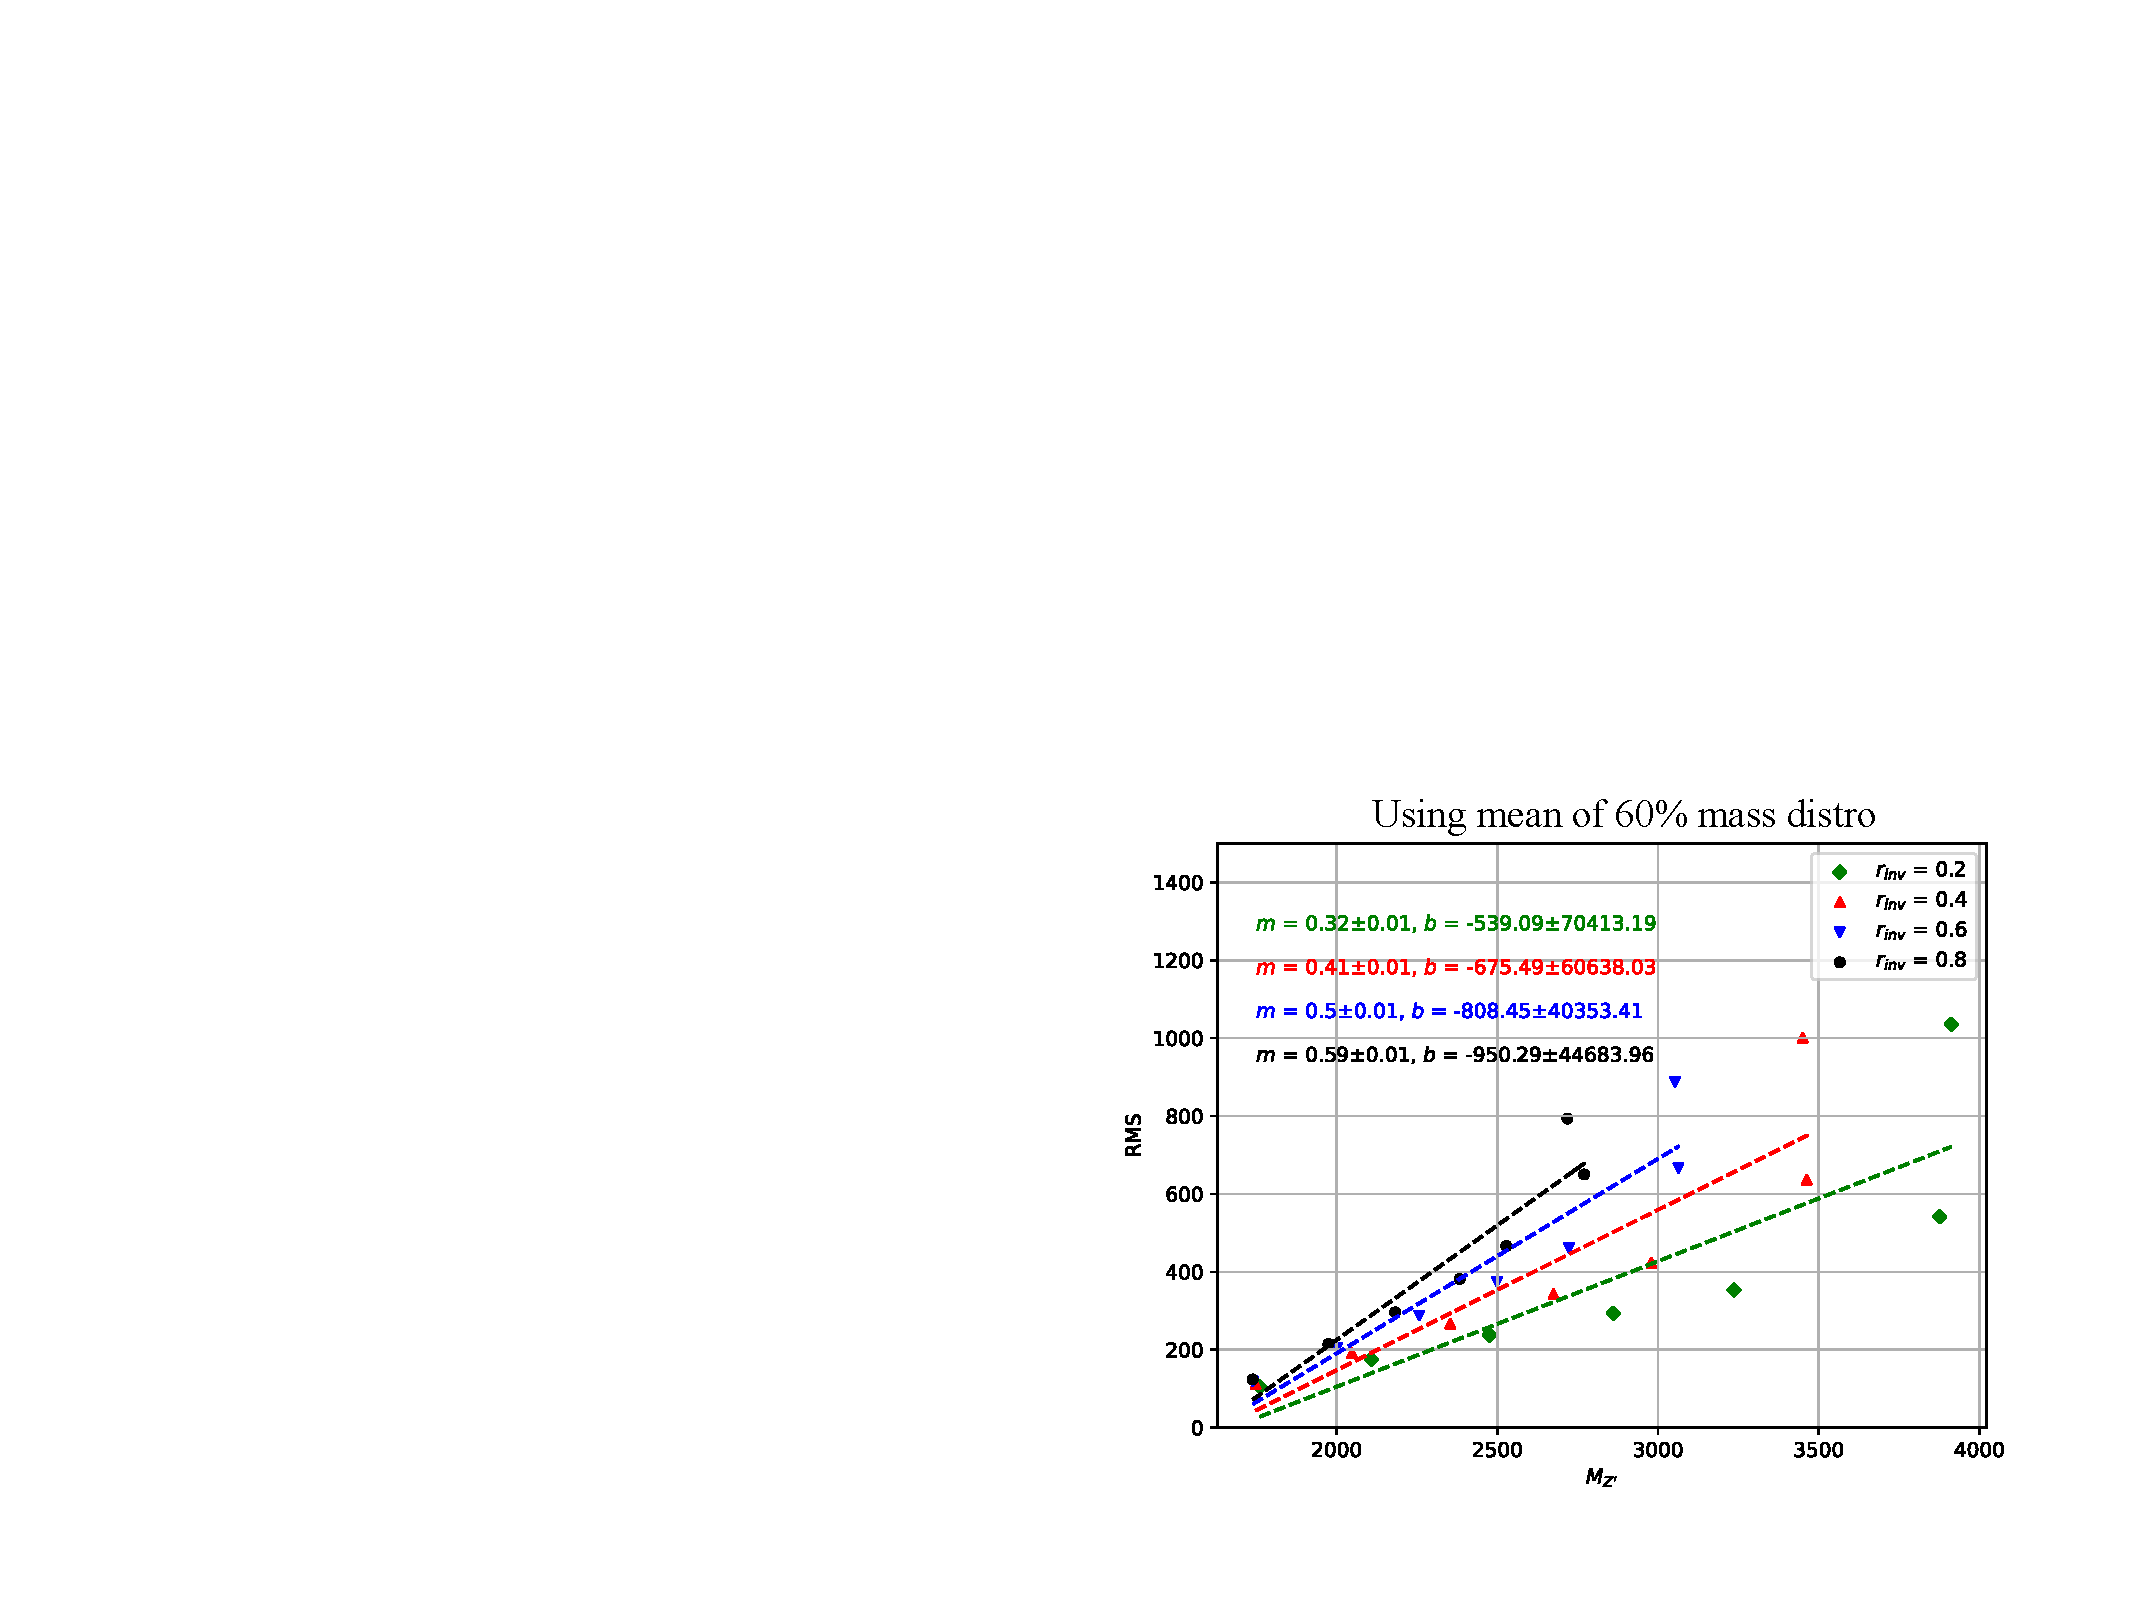
\includegraphics[width=0.52\textwidth]{figures/stats/linearfit_binning}
    \caption{Signal mass resolution for \mt~binning for the signal grid in (\rinv, mass) space.
    \label{fig:linearfit_binning}}
\end{figure}

A single \mt~binning for the final SR plotting and BumpHunting is determined by selecting a harmonized binning at low \mt~, and moving to wider bins at high \mt.
As for higher \rinv~signal points the mass resolution linear fit gives negative results, we require each bin to have a width of at least 100 GeV.
Figure~\ref{fig:bins_rinv} shows the resulting bins for each \rinv~category that comes from the mass resolution fits, with the addition of the minimum 100 GeV bin width requirement.
\begin{figure}[!htbp]
\centering
   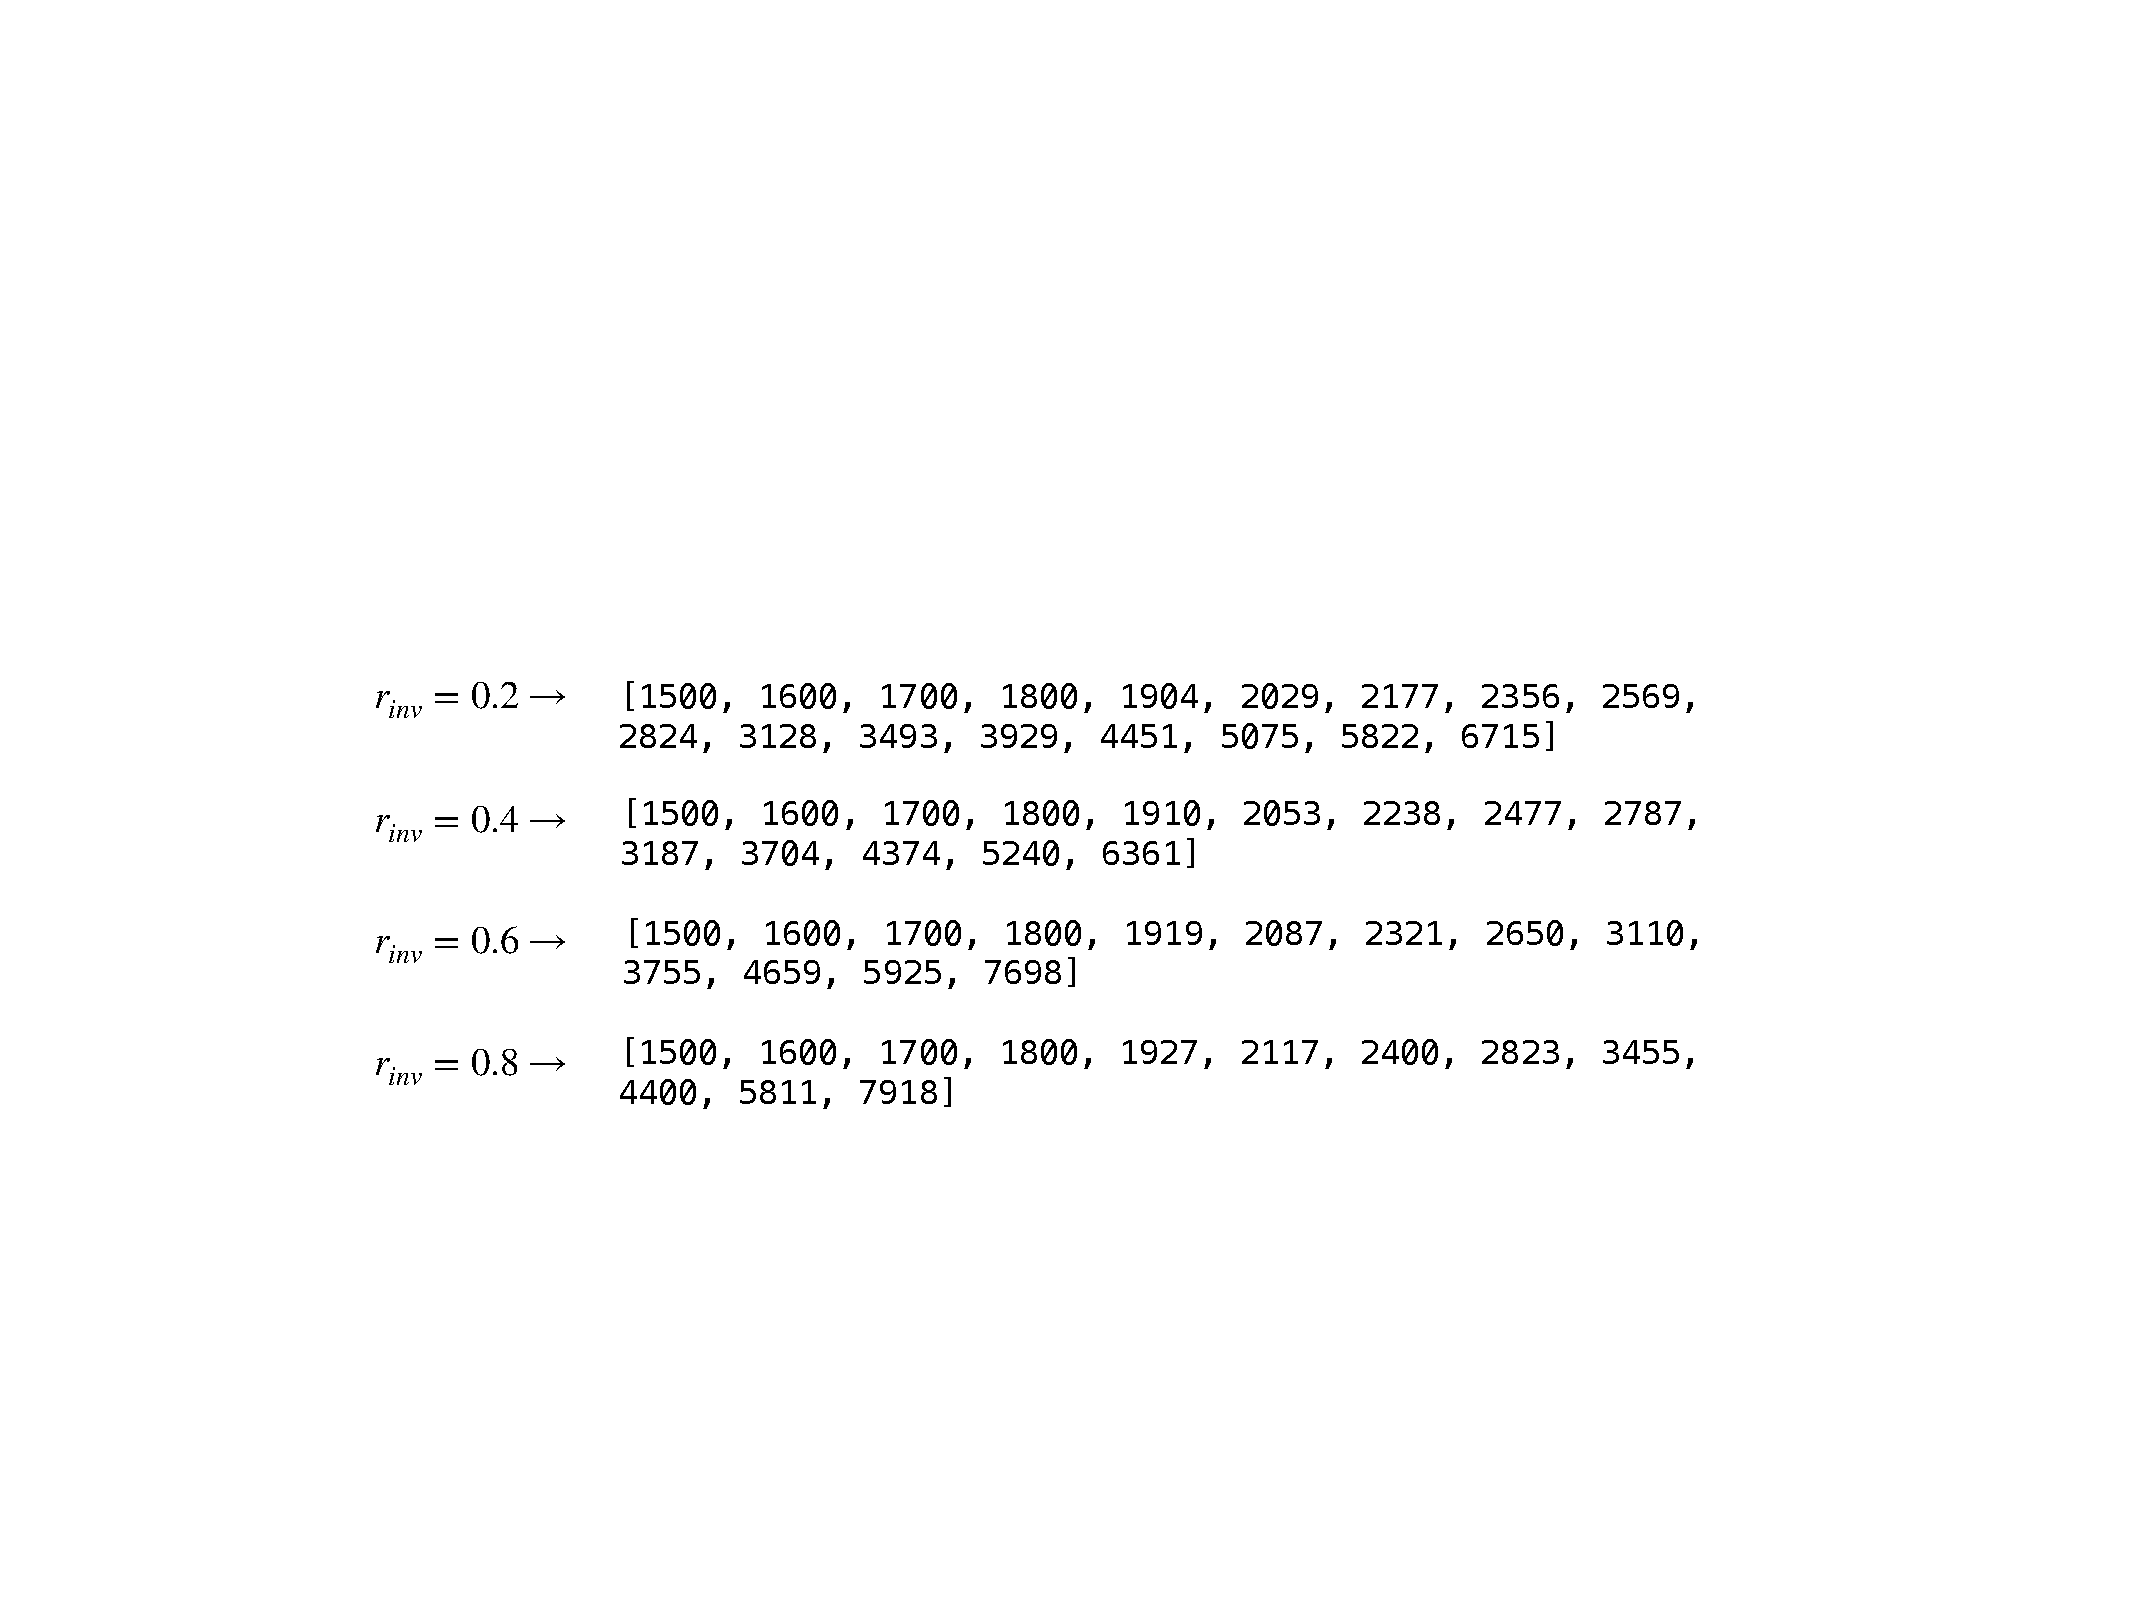
\includegraphics[width=0.82\textwidth]{figures/stats/bins_rinv}
    \caption{\mt~bins based on the signal mass resolution and the minimum 100 GeV width requirement, for each \rinv~signal category.
    \label{fig:bins_rinv}}
\end{figure}

In order to have a final \mt~binning that is not highly model-dependent, we consolidate these four different bins into a single binning which is provided below:

%\textbf{[1500, 1600, 1700, 1800, 1904, 2029, 2177, 2356, 2569, 2824, 3128, 3493, 3929, 4451, 5075, 6000]}
\textbf{[1500, 1600, 1700, 1800, 1900, 2025, 2175, 2350, 2575, 2825, 3125, 3500, 3925, 4450, 5075, 6000]}


%----------------------------------------------------------------------------------------
\subsubsection{BumpHunter Fits}
\label{subsec:bhfits}

Figure~\ref{fig:antelope_bh_crvr} shows the result of running BumpHunter over the CR and VR \mt~spectra, binned according to the signal mass resolution binning described above. 
The background estimation here is derived by fitting the ANTELOPE regions with the polynomial fit function, and sampling from this function to create a binned histogram.
We define a spurious signal as any BumpHunter fit finding an excess with p-value $<$ 0.01 (taken from other dijet analysis eg. Ref.~\cite{ATLAS:2023azi}).
No spurious signal is observed, and p-values indicate good agreement with the background estimation.
\begin{figure}[!htbp]
\centering
   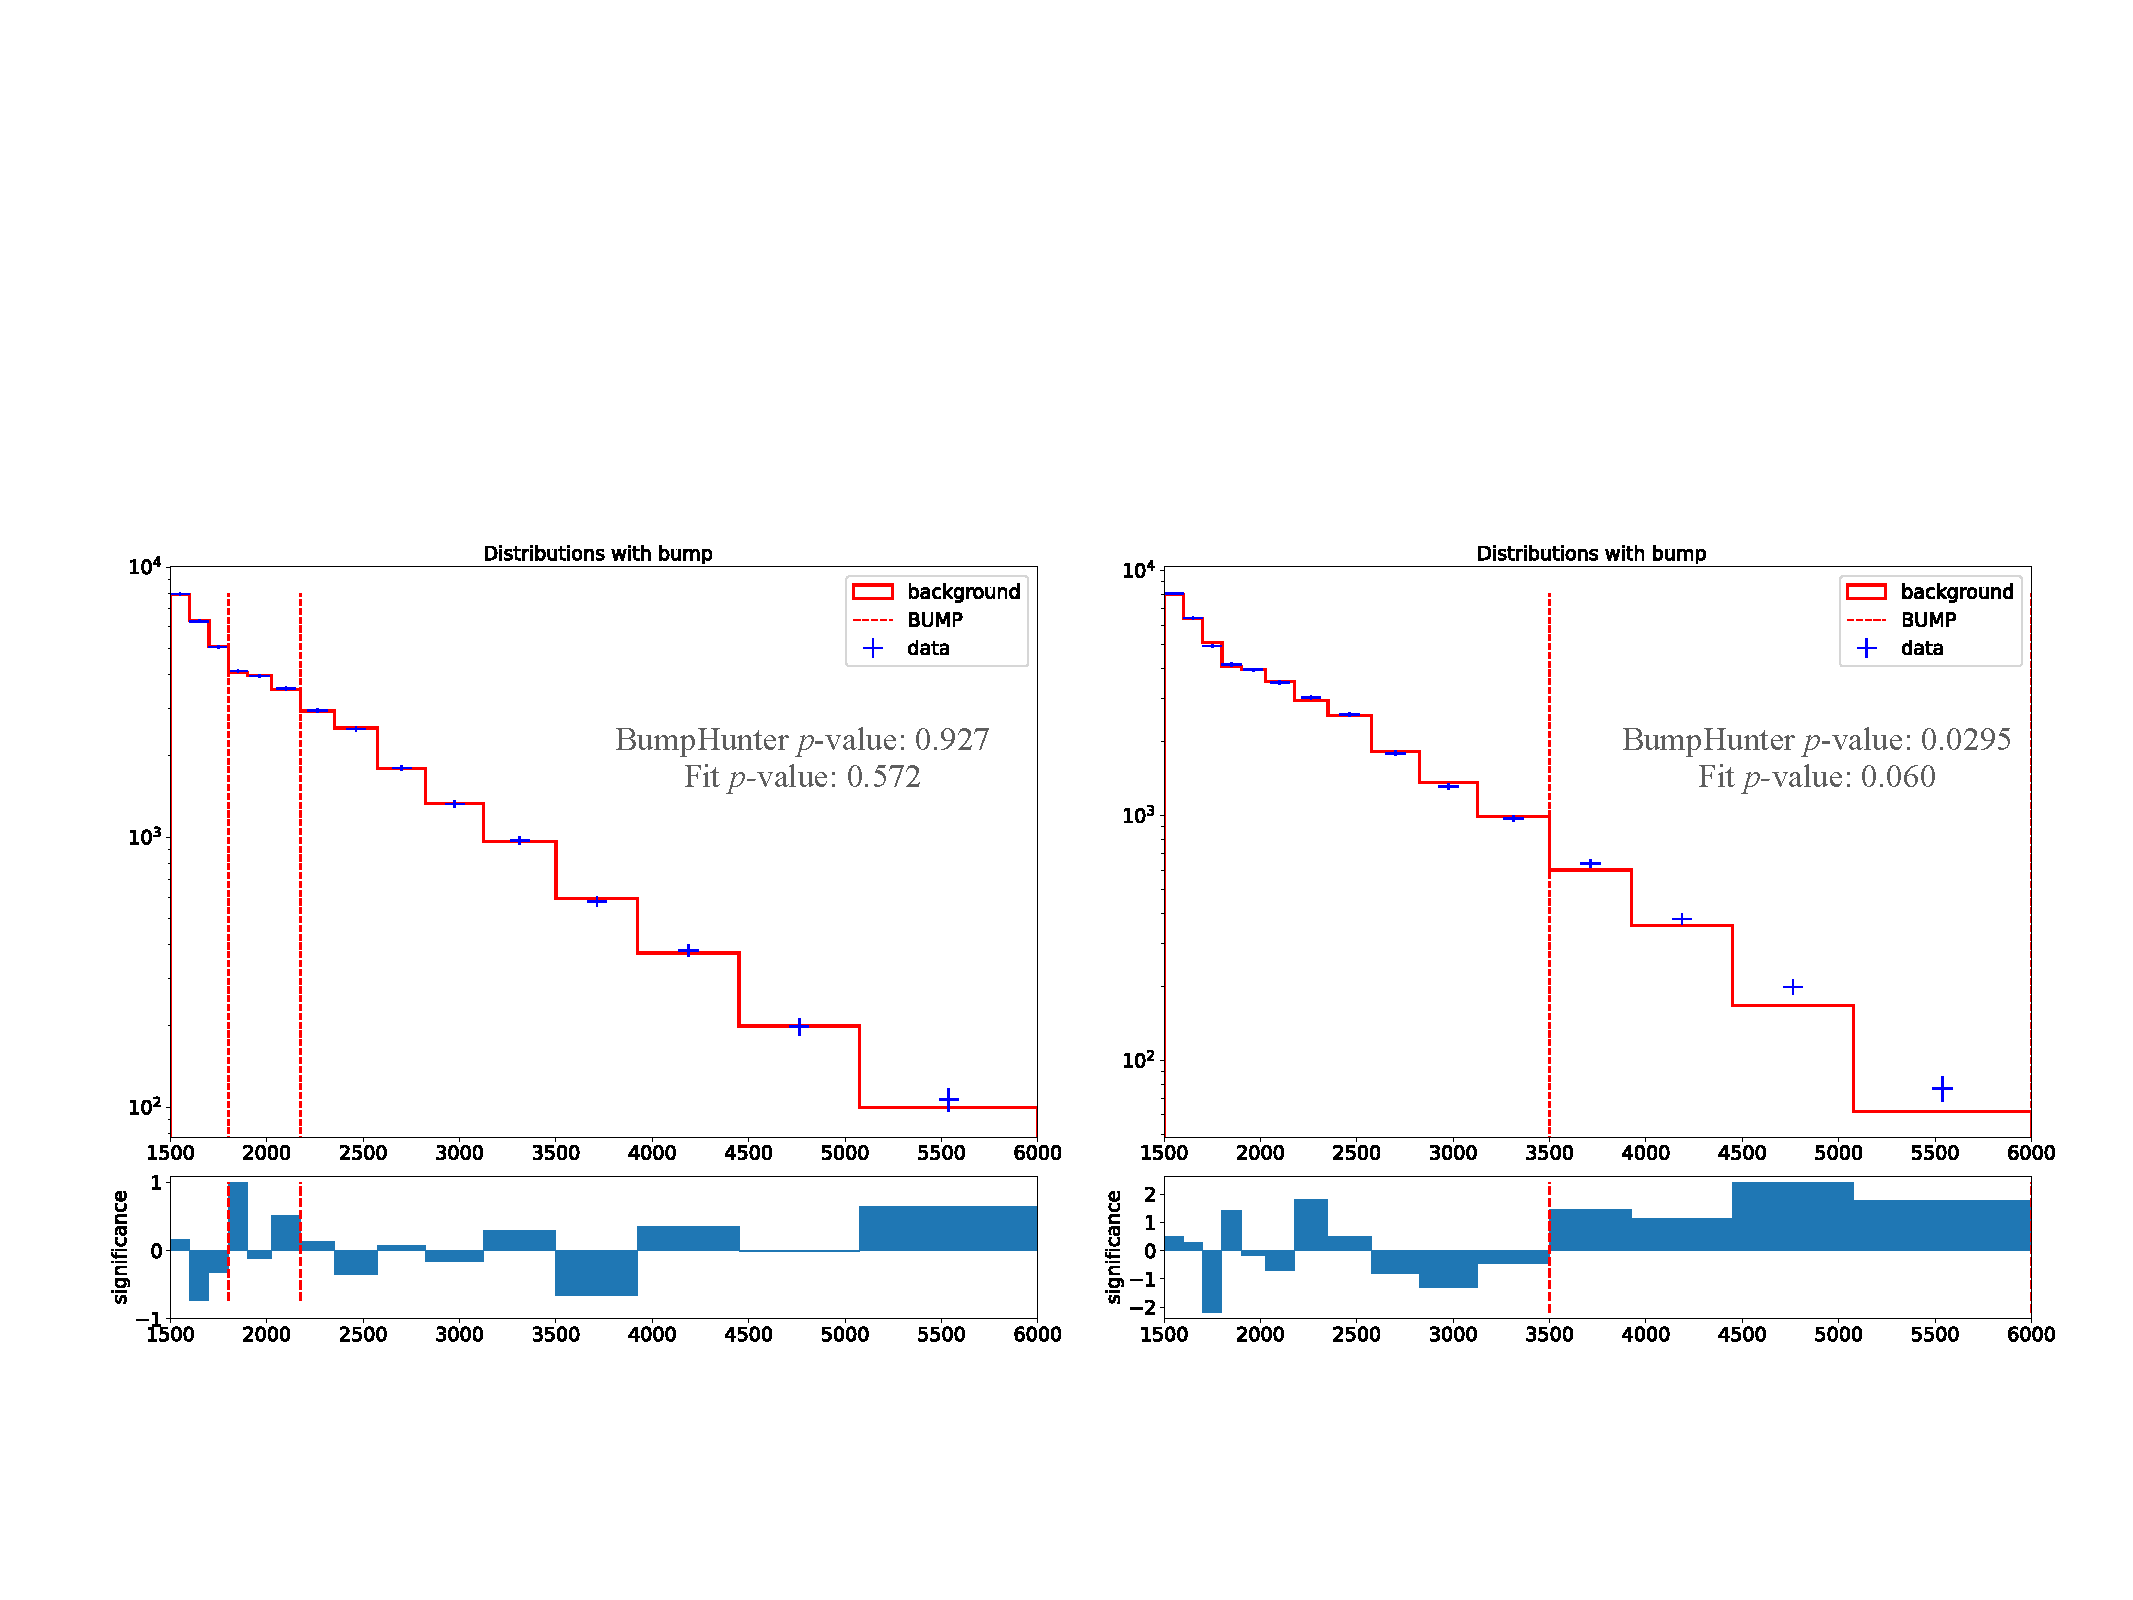
\includegraphics[width=0.95\textwidth]{figures/stats/antelope_bh_cr}
   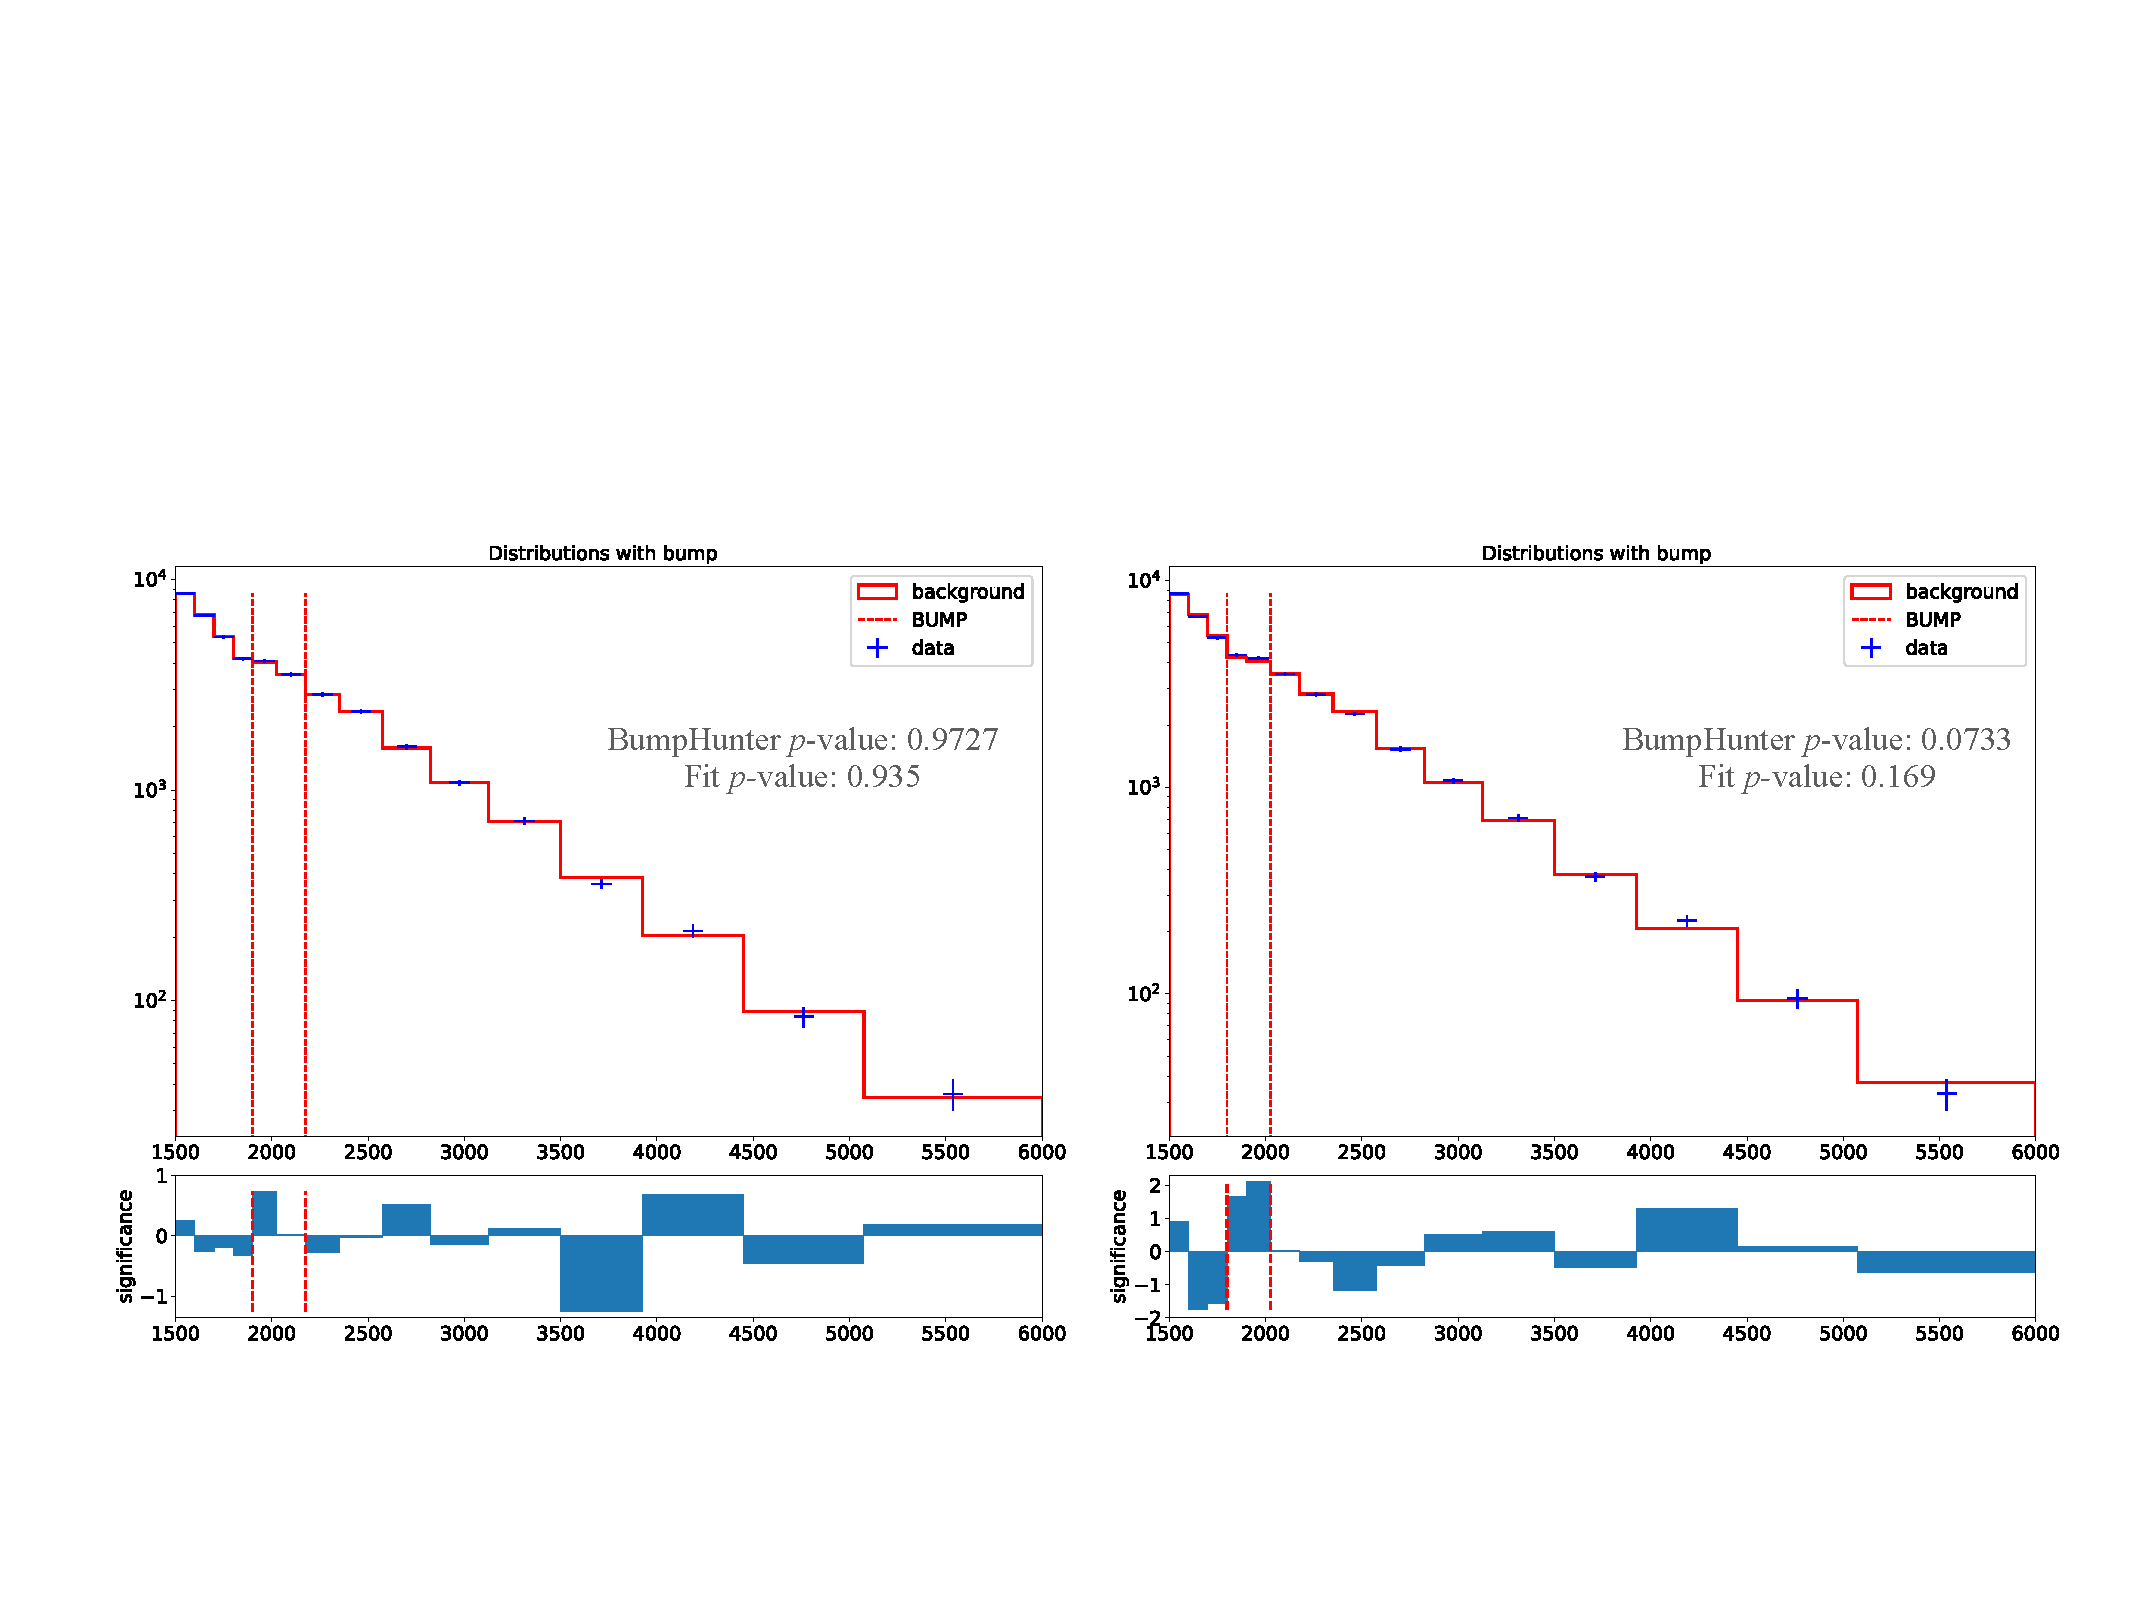
\includegraphics[width=0.95\textwidth]{figures/stats/antelope_bh_vr}
    \caption{BumpHunter fits on the ANTELOPE \mt~spectra for both the CR and VR. In a signal-depleted region, good agreement with the background estimation is observed.
    \label{fig:antelope_bh_crvr}}
\end{figure}

Figure~\ref{fig:bh_asimov_pvals} shows BumpHunter p-values over 100 Asimov trials
The same fit success criteria as the PFN region is applied: p-value  $>$ 0.001 and fit status succeeding (0 or 1).
In both cases, no spurious signals are found (p-value $<$ 0.01).
\begin{figure}[!htbp]
\centering
   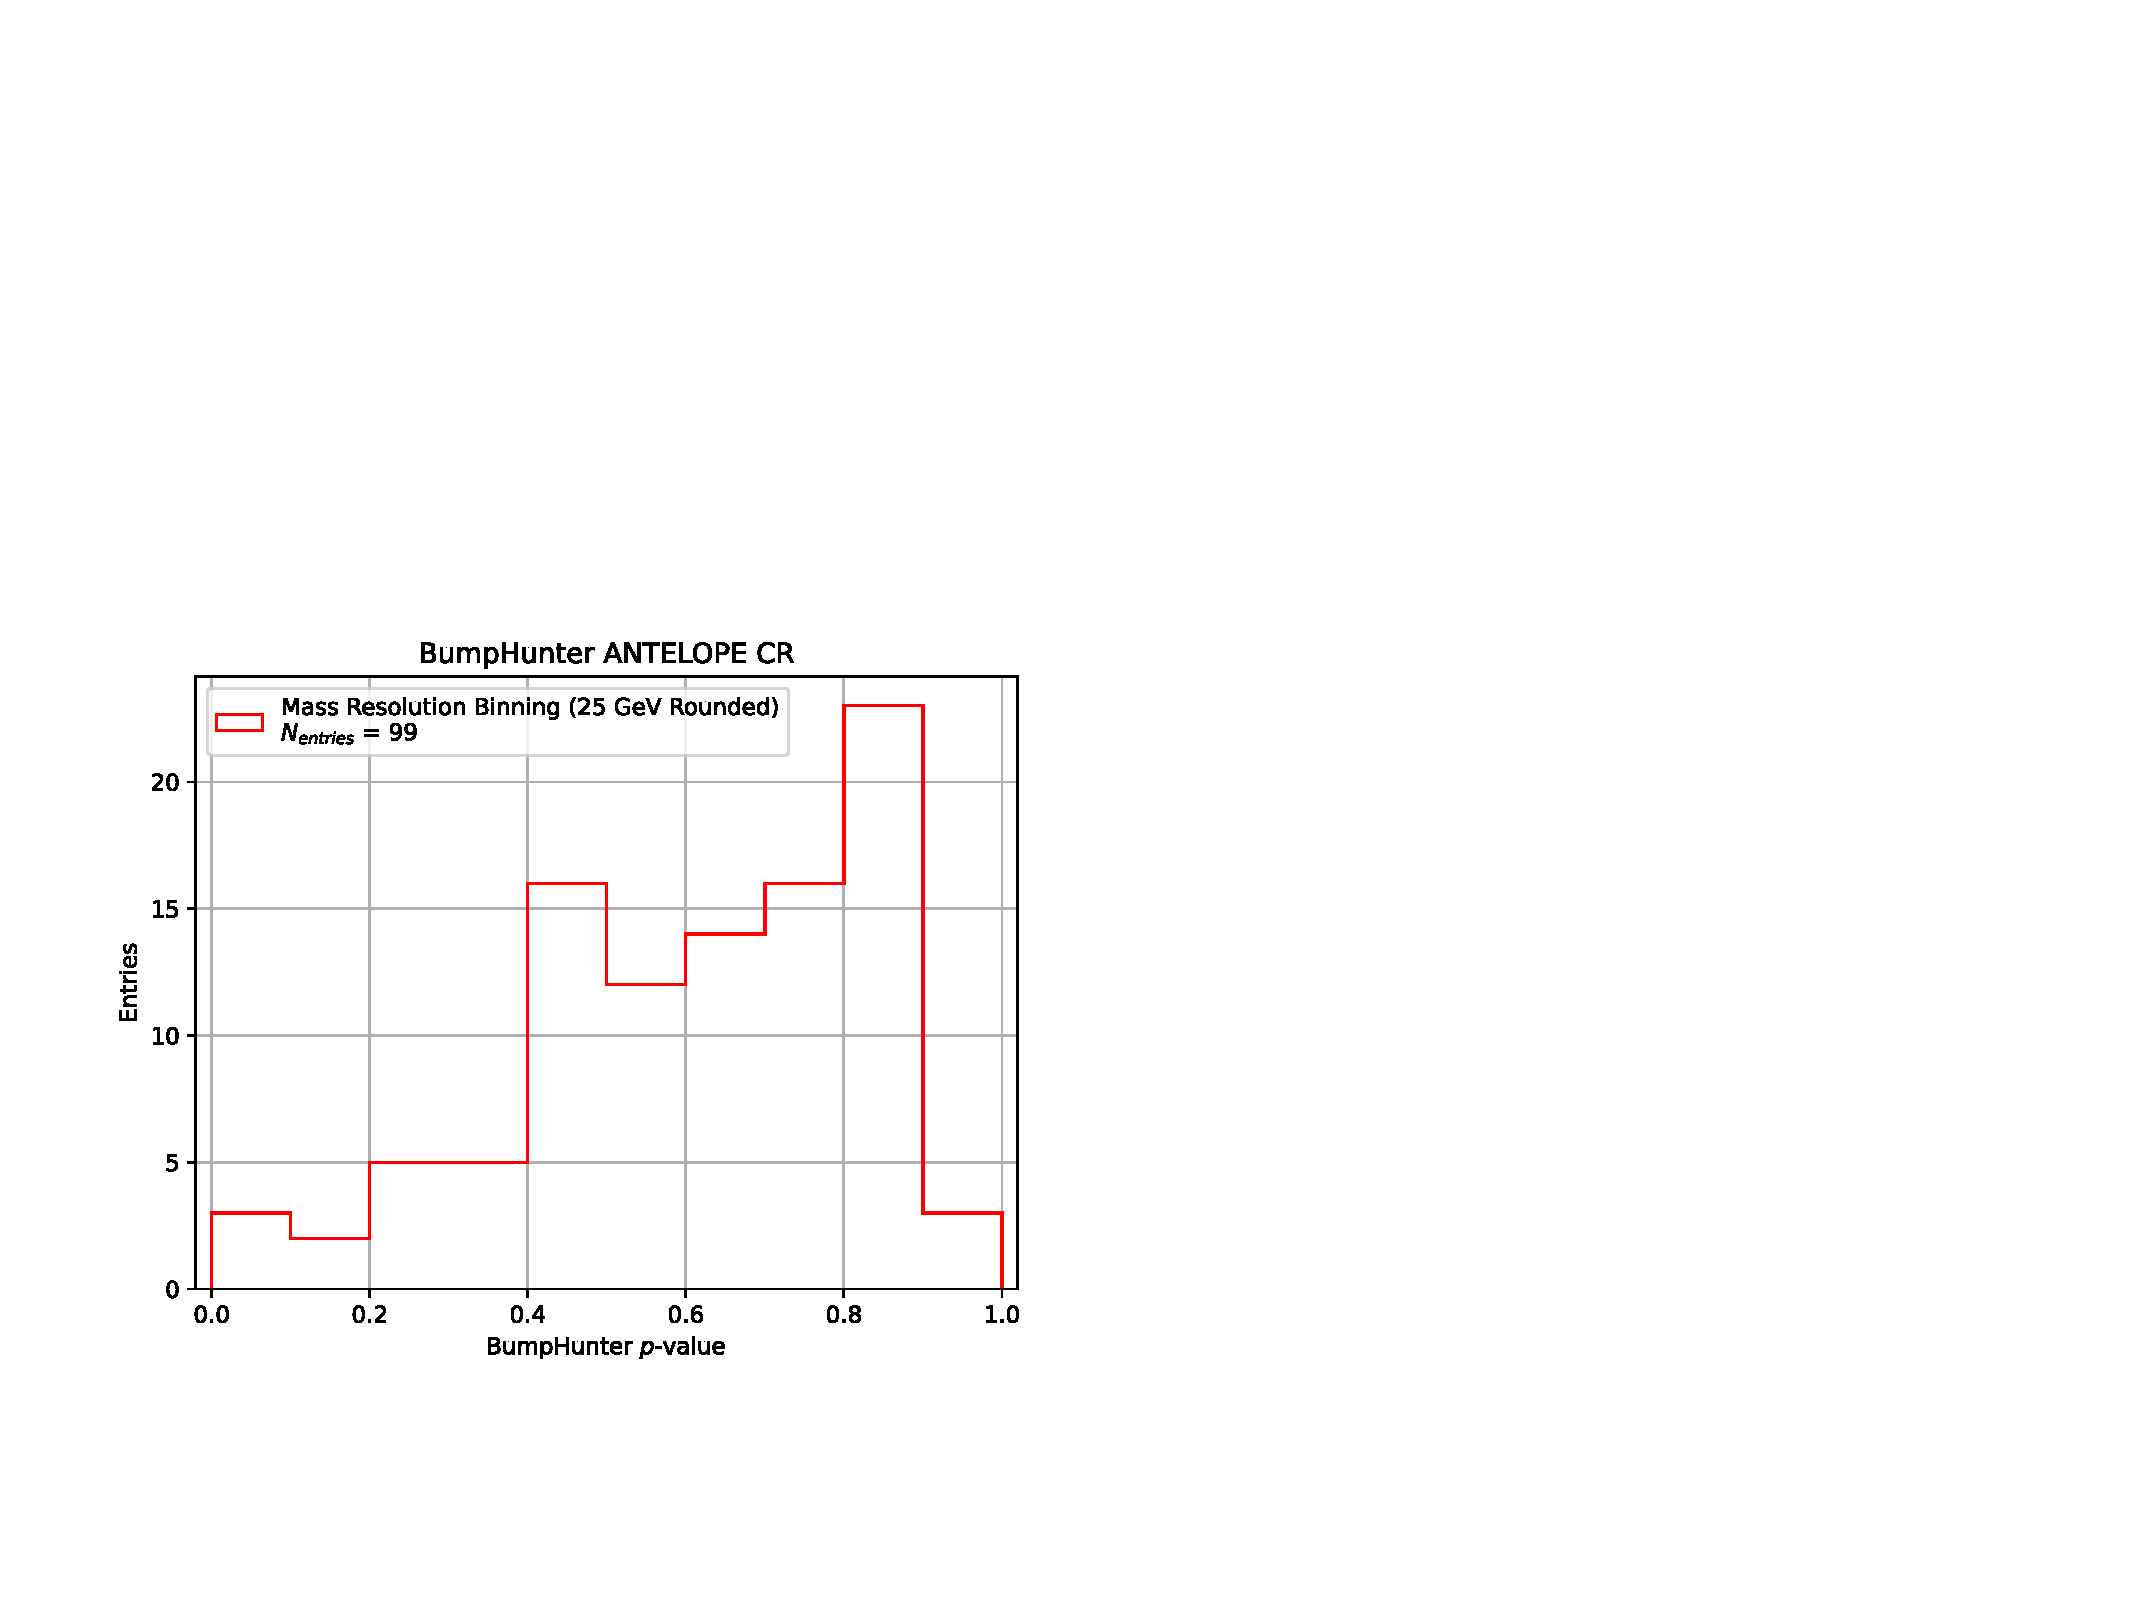
\includegraphics[width=0.45\textwidth]{figures/stats/bh_asimov_pvals_cr}
   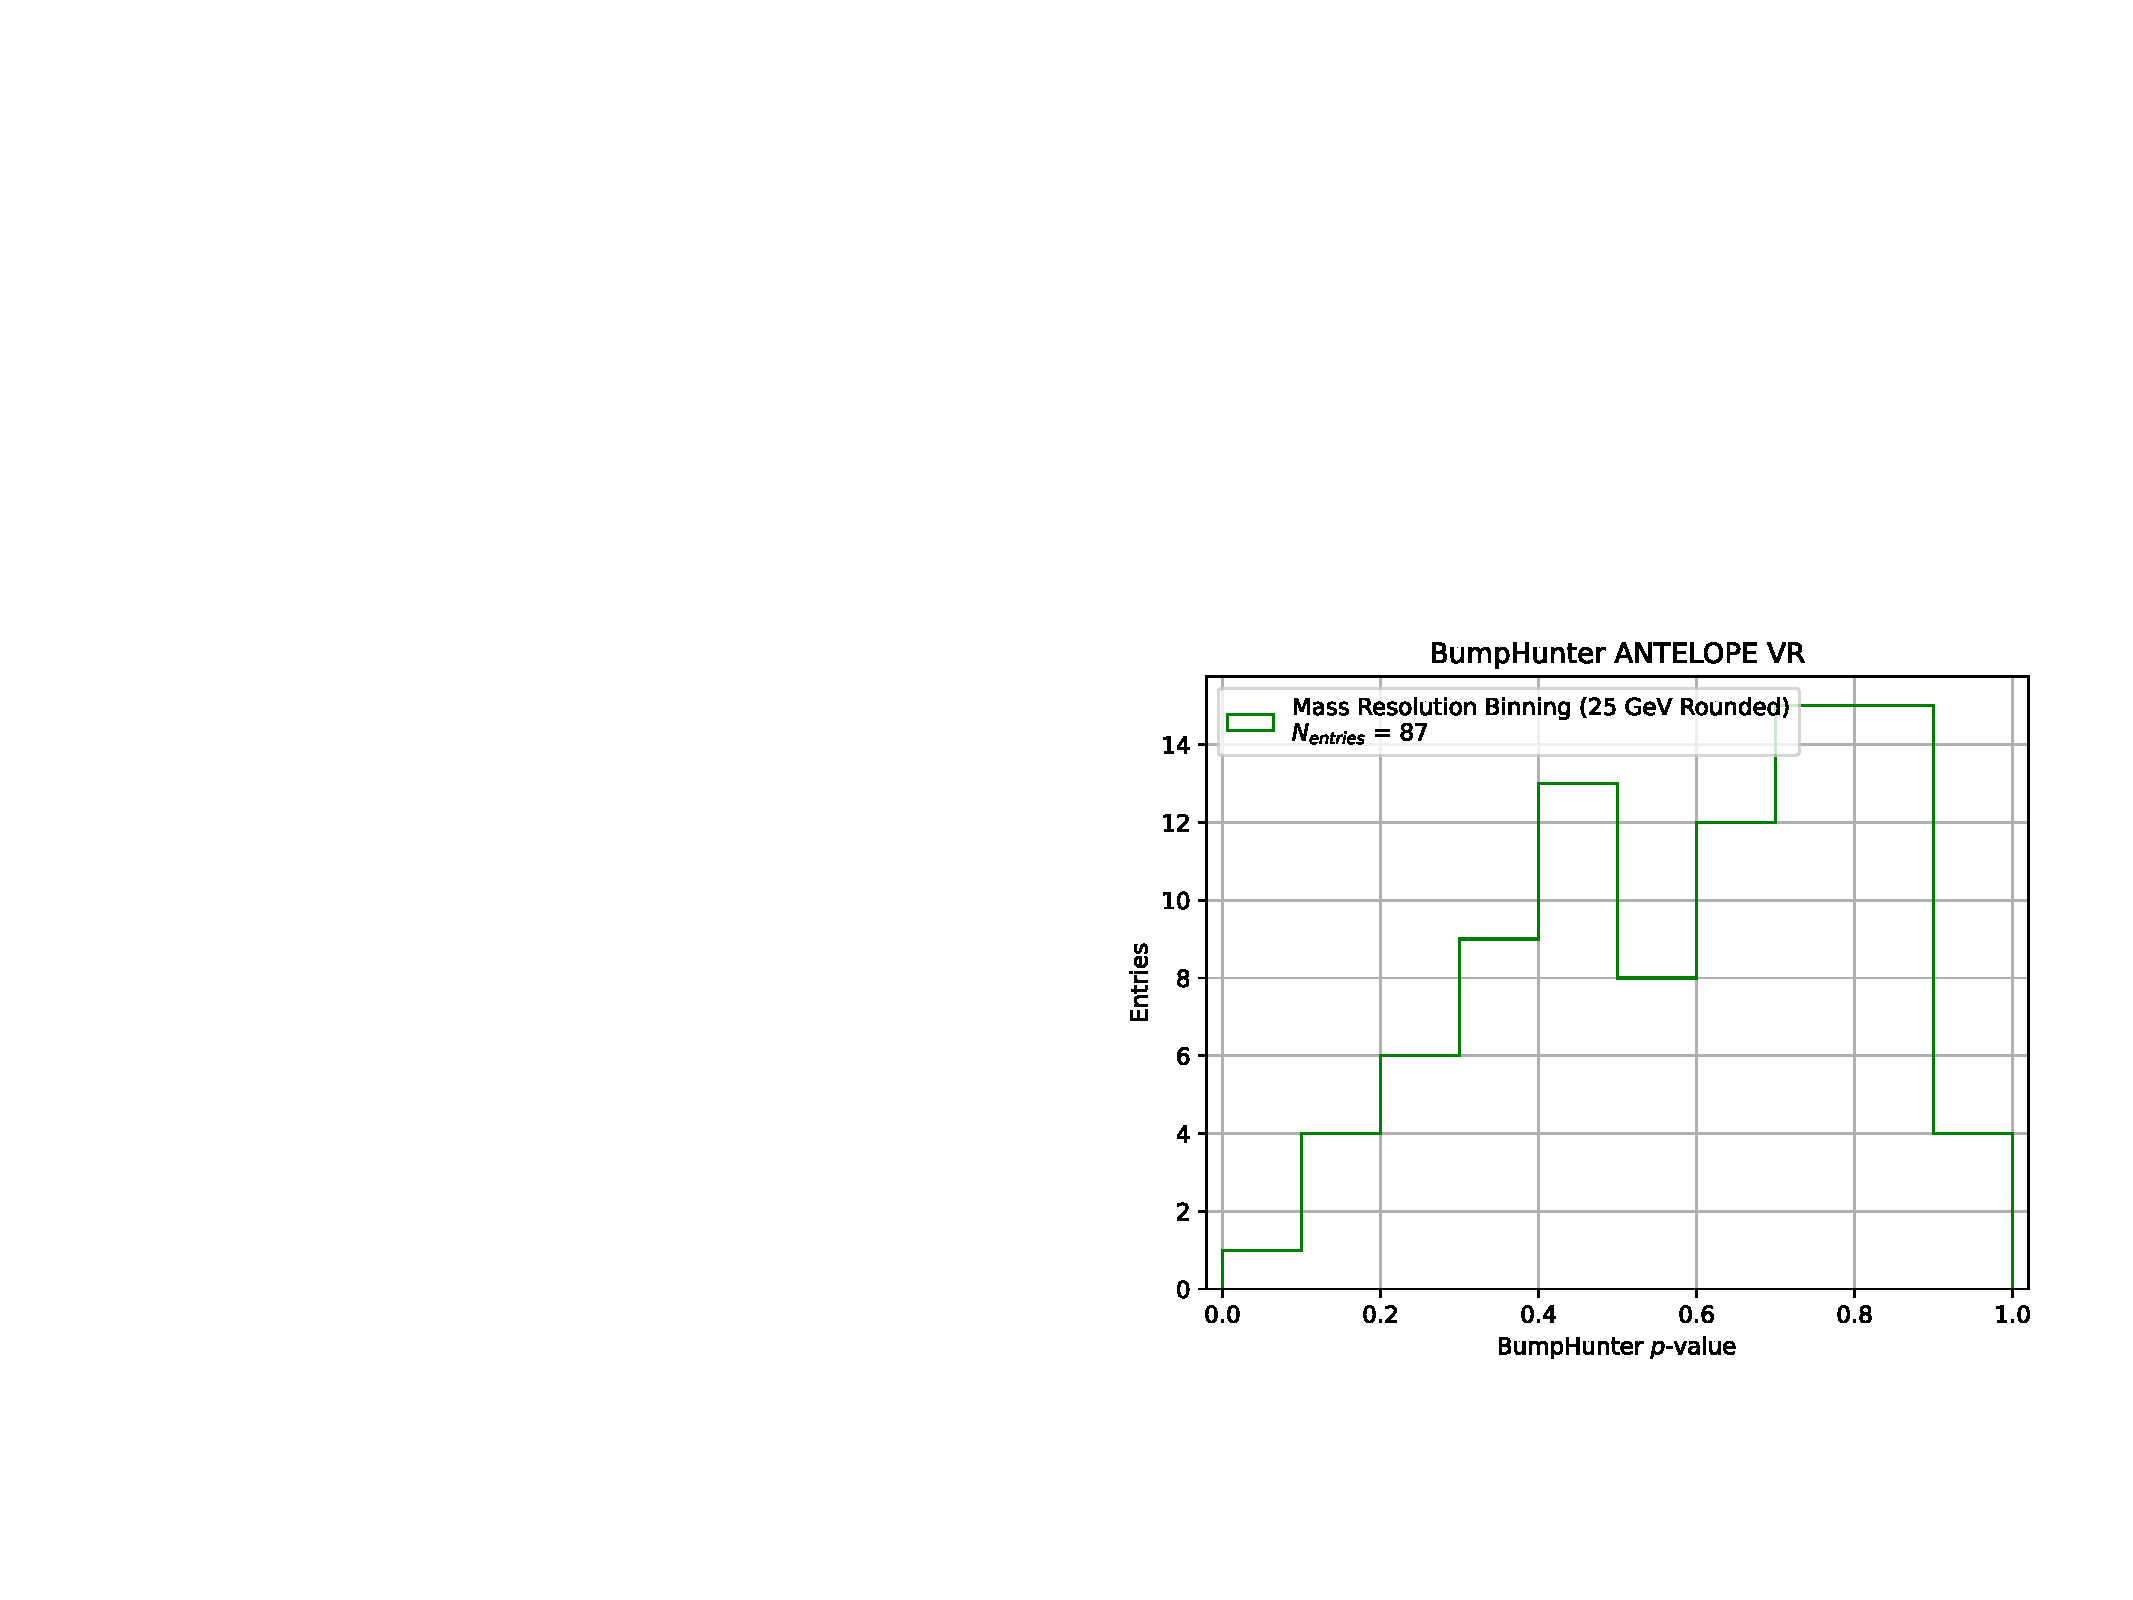
\includegraphics[width=0.45\textwidth]{figures/stats/bh_asimov_pvals_vr}
    \caption{BumpHunter p-values extracted for 100 Asimov toys for both the ANTELOPE CR (top) and VR (bottom) showing the highest (left) and lowest (right) p-value fits. The number of events in the histogram deviates from 100 based on failed background-only fits.
    \label{fig:bh_asimov_pvals}}
\end{figure}




